%% SafeStream-Redactor -- manuscript for the International Journal of Information Security (Springer)
%% Springer Nature LaTeX template (sn-jnl.cls), numbered references (sn-mathphys-num.bst).
%% Build: pdflatex main && bibtex main && pdflatex main && pdflatex main
%% Files: sn-jnl.cls, sn-mathphys-num.bst, refs.bib,
%%        fig_architecture.pdf, fig_memory.pdf, fig_accuracy.pdf, fig_scaling.pdf
\RequirePackage{fix-cm}
\RequirePackage{amsmath}
\RequirePackage{amsthm}% before the class, so sn-jnl defines its theorem styles
\documentclass[pdflatex,sn-mathphys-num]{sn-jnl}

\usepackage{graphicx}
\usepackage{multirow}
\usepackage{amssymb,amsfonts}
\usepackage[title]{appendix}
\usepackage{xcolor}
\usepackage{textcomp}
\usepackage{booktabs}
\usepackage{array}
\usepackage{xurl}
\usepackage{algorithm}
\usepackage{algorithmicx}
\usepackage{algpseudocode}
\usepackage{tikz}
\usetikzlibrary{arrows.meta,positioning,fit}

\theoremstyle{thmstyleone}
\newtheorem{theorem}{Theorem}
\newtheorem{lemma}{Lemma}
\newtheorem{corollary}{Corollary}
\theoremstyle{thmstylethree}
\newtheorem{definition}{Definition}
\newtheorem{assumption}{Assumption}
\renewcommand{\theassumption}{A\arabic{assumption}}

\hypersetup{bookmarksdepth=2}
%% sn-jnl draws its (empty) running head as \vbox to 0pt{\vspace*{-48pt}...}, which
%% raises an "Underfull \vbox ... while \output is active" warning on every page.
%% The head prints nothing, so an empty head gives the same page without the warning.
\makeatletter
\def\ps@headings{\def\@oddfoot{\hfill\thepage\hfill}\let\@evenfoot\@oddfoot
  \let\@oddhead\@empty\let\@evenhead\@empty\let\@mkboth\markboth}
\def\ps@titlepage{\let\@oddhead\@empty\let\@evenhead\@empty
  \def\@oddfoot{\vbox to 18pt{\vfill\reset@font\rmfamily\hfil\thepage\hfil}}\def\@evenfoot{}}
\makeatother
\pagestyle{headings}
\emergencystretch=2em

\newcommand{\ns}{$^{\dagger}$}
%% point estimate with its interval stacked underneath, so no interval wraps or clips
\newcommand{\pc}[2]{\begin{tabular}[t]{@{}l@{}}#1\\[-1pt]{[}#2{]}\end{tabular}}

\begin{document}
\raggedbottom

\title[Bounded-memory streaming redaction with a whole-document equivalence guarantee]{Bounded-memory streaming redaction of personal data and credentials with a whole-document equivalence guarantee}

\author[1]{\fnm{Mounish} \sur{Senisetty}}\email{am.ai.u4aid23058@am.students.amrita.edu}
\author[1]{\fnm{Sandhiya} \sur{Kennedy}}\email{am.ai.u4aid23056@am.students.amrita.edu}
\author[1]{\fnm{Ashrith Reddy} \sur{N}}\email{am.ai.u4aid23014@am.students.amrita.edu}
\author*[1]{\fnm{Parvathy} \sur{R}}\email{parvathyr@am.amrita.edu}

\affil*[1]{\orgdiv{Amrita School of Computing}, \orgname{Amrita Vishwa Vidyapeetham}, \orgaddress{\city{Amritapuri}, \country{India}}}

\abstract{Logs and data exports carry personal data and credentials and are often too large to hold in memory. Processing them in chunks adds a silent failure: a value straddling a chunk boundary reaches the detector in two halves and is written out in the clear. SafeStream-Redactor, a local redaction engine, treats chunking as a correctness problem. Each detector declares the longest span it emits and the context it reads. We show that an overlap as long as the longest span can still leak, and prove that if the overlap covers every detector's span plus its right context, the streamed output equals a whole-document pass, parallel output equals sequential output or falls back to it, and the working buffer is independent of input size; the engine enforces this overlap. Naive 1\,KiB chunking leaked 237 RedactionBench values that a whole-document pass redacts, and overlapping windows still leaked some; SafeStream matched the whole-document output under every chunking tried. Streaming added 8.4--8.54\,MiB of memory from 8\,MiB to 2\,GiB, against 904.6\,MiB for whole-document redaction of 32\,MiB; throughput reached 10.5\,MB/s with one worker and 41.1\,MB/s with four. On held-out data the pattern tiers fully redacted 0.437 of credentials, against 0.311 for gitleaks and 0.270 for TruffleHog; the gitleaks margin survives clustered resampling and disabled filters. Detection remains incomplete: no configuration fully protected more than 17.9\% of RedactionBench documents, and two of the three corpora are synthetic.}

\keywords{Data redaction, Secret detection, Data loss prevention, Streaming algorithms, Bounded memory, Personally identifiable information}

\maketitle

%% ===================================================================
\section{Introduction}\label{sec:intro}

Text artefacts that leave an organisation, such as an application log attached to a support ticket, a database export handed to an analyst, or a packet capture shared with a vendor, routinely carry two classes of sensitive value: personal data (e-mail addresses, telephone and card numbers, national identifiers, names) and credentials (application programming interface keys, access tokens, private keys, passwords). Data-loss-prevention systems inspect such content before it crosses a boundary \cite{alneyadi2016dlp}, and measurement studies show that credentials leak into shared artefacts at scale \cite{meli2019git,krause2023pushed}.

Two families of tools address the problem. Personal-data engines such as Microsoft Presidio \cite{presidio} combine pattern recognisers with a statistical named-entity model but ship no credential recognisers. Secret scanners such as gitleaks \cite{gitleaks} and TruffleHog \cite{trufflehog} target credentials in source repositories, and their accuracy varies widely across secret types \cite{basak2023comparative}. The artefacts that most need redaction are often too large to analyse in one call, so they are processed in pieces. A chunked redactor can then fail silently: a value that straddles a chunk boundary is presented to the detector in two halves, neither of which matches, and both halves are written out in the clear. The same problem is long established in network security, where signatures split across packets motivated stream reassembly in intrusion detection \cite{ptacek1998insertion} and streaming modes in regular-expression engines \cite{wang2019hyperscan,intel2019hyperscanintro}. In redaction, however, detectors read context around a match (``Patient ID:'' before a number, a key name before a token), confidences are adjusted by neighbouring text, and overlapping detections are merged before the text is rewritten. Overlapping windows are the obvious remedy, but how much overlap is enough depends on all of these, and the obvious answer, an overlap as long as the longest match, is wrong: a match whose right context is cut off at the window edge can be rejected there, so the boundary does not retreat out of it and its first part is emitted in the clear. None of the redaction or secret-scanning systems we examined states when its chunked output equals its whole-document output.

This paper answers that question for a concrete system, SafeStream-Redactor (hereafter SafeStream). Its contributions are the following.
\begin{enumerate}
\item \textbf{A tight, per-detector overlap condition for context-dependent redaction.} Every detector $d$ declares an upper bound $L_d$ on the span it can emit and bounds $C_{\mathrm{left},d}$ and $C_{\mathrm{right},d}$ on the context it reads (Assumptions~\ref{as:span} and~\ref{as:ctx}). We prove that an overlap $w \ge \max_d \max(L_d + C_{\mathrm{right},d},\, C_{\mathrm{left},d})$ makes the streamed output equal to the whole-document output for every chunking, and show that the term $L_d + C_{\mathrm{right},d}$ cannot be dropped: an overlap of $\max_d L_d$, the natural choice, can leak (Section~\ref{sec:formal}). We also measure the failure the condition prevents: on the test corpora, naive chunking leaked up to 237 gold values that a whole-document pass redacts, and overlapping windows still leaked some, while SafeStream's output was identical to the whole-document output under every chunking tried (Section~\ref{sec:equiv}). The underlying locality argument is standard; what is new is the condition for pipelines whose detectors read context on both sides, adjust confidences and resolve overlaps jointly, which pattern-matching engines that carry automaton state across blocks do not address.
\item \textbf{A guarantee enforced by the code, not chosen by hand.} The engine computes the condition from the detectors' declarations and refuses to run with a smaller overlap; regression and differential tests check that the declarations hold. For the default pipeline the requirement is exactly the default overlap of 8192 characters.
\item \textbf{Parallel redaction that cannot lose or duplicate text.} A seam protocol between worker processes makes the parallel output equal to the sequential output under the same condition, and falls back to sequential processing on any disagreement, so no character is lost or emitted twice whatever the detectors do (Appendix~\ref{app:proofs}).
\item \textbf{Bounded memory, measured.} The working buffer is bounded independently of input size, and peak memory stays flat across a 256-fold range of input sizes, where whole-document redaction needs about 28 times the input size (Section~\ref{sec:memory}).
\item \textbf{A detection evaluation that separates robust from fragile margins.} Equivalence says nothing about how good the detectors are. We evaluate them on held-out test splits against Presidio and two secret scanners, with paired bootstrap intervals at the document, cluster and two-stage levels, a scanner sensitivity run with false-positive filters disabled, an ablation and a contamination analysis (Sections~\ref{sec:setup} and~\ref{sec:results}). Two margins survive every check: a higher fully redacted rate for credentials than gitleaks, and higher character F1 than Presidio with the same spaCy model. Others do not, and we report them as such.
\end{enumerate}

Two scope limits are stated at the outset. First, the guarantee concerns equivalence rather than accuracy: streaming does not improve detection, it makes the streamed result the same as the whole-document result, so every detection error of the whole-document pipeline is also an error of the streamed one. Second, the evaluation has known weaknesses that we quantify rather than omit: one corpus, RedactionBench, was inspected during rule development (Section~\ref{sec:contam}); two corpora are synthetic; and fewer than one RedactionBench document in five was fully protected by any configuration we evaluated (Section~\ref{sec:noleak}). Section~\ref{sec:discussion} states when the approach is useful despite these limits and what evidence a deployment would need.

%% ===================================================================
\section{Background and related work}\label{sec:related}

\paragraph{Personal-data detection and de-identification}
Rule-based de-identification of clinical text dates back to lookup tables and regular expressions applied to nursing notes \cite{neamatullah2008deid}; Philter refined the approach on a large annotated clinical corpus \cite{norgeot2020philter}. The 2014 i2b2/UTHealth shared task established annotated corpora and evaluation practice \cite{stubbs2015annotating}, and recurrent neural networks reached strong results on them \cite{dernoncourt2017deid}. Presidio \cite{presidio} combines pattern recognisers with spaCy or transformer models and ships an evaluation toolkit with a synthetic dataset \cite{presidioresearch}. Lison et al.\ argue that sequence labelling alone does not amount to anonymisation and call for explicit disclosure-risk measures \cite{lison2021anonymisation}; the Text Anonymization Benchmark operationalises this for court judgments \cite{pilan2022tab}. Named-entity recognition underpins the free-text part of these systems, from the CoNLL-2003 shared task \cite{tjongkimsang2003conll} to transformer encoders \cite{devlin2019bert,sanh2019distilbert} and generalist span models \cite{zaratiana2024gliner}. Pseudonymisation with a keyed hash such as HMAC \cite{rfc2104} preserves referential integrity but reveals equality between values, so it is not anonymisation in the sense of $k$-anonymity \cite{sweeney2002kanonymity}. Redaction as studied here is narrower than anonymisation: it removes spans that detectors recognise and makes no claim about re-identification from what remains.

\paragraph{Credential and secret detection}
Meli et al.\ measured secret leakage across public GitHub repositories \cite{meli2019git}. Approaches range from vendor-specific regular expressions \cite{sinha2015secretkey} to machine-learned filters that reduce false positives \cite{saha2020secrets} and neural detectors for free-form passwords \cite{feng2022passfinder}. SecretBench provides a labelled corpus of candidate secrets \cite{basak2023secretbench}, and a comparison of nine tools attributed false positives to generic patterns and entropy heuristics and false negatives to missing rules \cite{basak2023comparative}. Krause et al.\ studied how developers handle leaked secrets \cite{krause2023pushed}. Shannon entropy \cite{shannon1948} is the usual signal for undocumented high-entropy secrets. The Nosey Parker rule set \cite{noseyparker} supplies the labelled examples we evaluate on.

\paragraph{Detection across segment boundaries}
That a pattern split across units of input can evade a detector is well known in network security: Ptacek and Newsham showed that intrusion detectors which do not reconstruct streams as the end host does can be evaded \cite{ptacek1998insertion}, and Hyperscan \cite{wang2019hyperscan} provides a streaming mode whose matches do not depend on how the data is split into blocks \cite{intel2019hyperscanintro}. These systems carry automaton state across boundaries, which makes pattern matching exact but says nothing about what happens after a match: validators, context-dependent confidences and joint overlap resolution all read text the automaton has already consumed. A redaction pipeline differs in three ways that affect correctness: detectors consult bounded context on both sides of a match, confidences depend on nearby text, and overlapping detections are resolved jointly before the output is rewritten. Overlapping windows are a common way to process long inputs, and the stream model \cite{muthukrishnan2005streams} formalises computation in bounded memory; linear-time regular-expression matching goes back to Thompson \cite{thompson1968regex}. Among the redaction, de-identification and secret-scanning systems cited above, we found none that states when chunked output equals whole-document output or how the overlap must be sized. We do not claim that the underlying locality argument is new; the contribution is its instantiation and enforcement for context-dependent redaction.

%% ===================================================================
\section{Problem statement and threat model}\label{sec:problem}

\begin{definition}[Detections and redaction]\label{def:det}
A text $T$ is a finite character string, and $T[a{:}b]$ is its half-open substring. A \emph{detection} is a tuple $(i, j, \tau, c)$ with $0 \le i < j \le |T|$: a half-open span, an entity type and a confidence in $[0,1]$. Each detection is produced by one detector $d$ of a finite set $\mathcal{D}$. A \emph{pipeline} $\Pi$ maps $T$ to a set of pairwise-disjoint detections. \emph{Redaction} rewrites $T$ by replacing each span in $\Pi(T)$ according to a policy (replace, mask, hash, keyed pseudonym or encryption). The replacement of a span depends only on its type and its text, so redaction is a deterministic function of $T$ and $\Pi(T)$ that acts on each span separately.
\end{definition}

\begin{definition}[Leak]
Given a set $G$ of gold sensitive spans for $T$, a \emph{leak} is any character of a span in $G$ that is not covered by a span in $\Pi(T)$. A gold span with at least one uncovered character is \emph{leaked}, because a partly visible card number or key can often be reconstructed or narrowed.
\end{definition}

\paragraph{Adversary and setting}
The adversary is a later reader of the redacted output, for example the recipient of a shared log. The input may be larger than memory and arrive as an arbitrary sequence of chunks. The system runs locally and makes no network calls, so the unredacted text does not leave the host.

\paragraph{What is in scope}
(i) That chunked and parallel processing introduce no leak beyond those of the whole-document pipeline; (ii) bounded working memory; (iii) the detection quality of the whole-document pipeline, measured empirically.

\paragraph{What is out of scope}
Detection completeness: the pipeline misses values its detectors do not recognise, and the guarantee does not change that. Adversarial evasion: an author who encodes, splits or obfuscates a secret on purpose is not modelled. Inference from residual text: quasi-identifiers and context that remain after redaction may still allow re-identification \cite{lison2021anonymisation,sweeney2002kanonymity}. Side channels such as output length. Bounded memory is a resource property, not a security property.

%% ===================================================================
\section{Design}\label{sec:method}

\begin{figure*}[t]
\centering
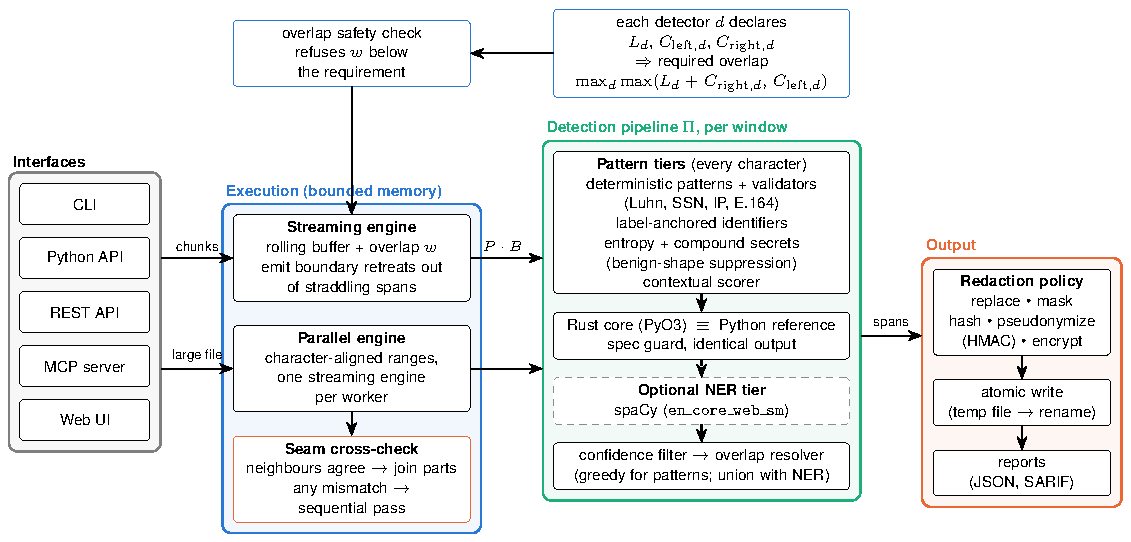
\includegraphics[width=\textwidth]{fig_architecture.pdf}
\caption{System architecture. Interfaces feed text to the streaming engine or, for a large file, to the parallel engine, whose workers each run a streaming engine and whose seams are cross-checked. Each window passes through the detection pipeline $\Pi$: the pattern tiers run on every character, on the Rust core or the identical Python reference. The dashed named-entity tier (spaCy) is optional. The resolver produces disjoint spans, which the redaction policy rewrites and an atomic write commits. The overlap $w$ is checked against the span and context bounds the active detectors declare.}\label{fig:pipeline}
\end{figure*}

Figure~\ref{fig:pipeline} shows the architecture. The reference pipeline $\Pi$ runs every configured detector on a text, adjusts confidences with a bounded contextual scorer, drops detections below a threshold (0.5 by default) and resolves overlaps into a disjoint set.

\subsection{Detection tiers}\label{sec:tiers}

\paragraph{Deterministic patterns with validators}
Credential formats with a fixed shape (cloud access keys, provider tokens, JSON Web Tokens, PEM private-key blocks) and structured personal data (e-mail, telephone, card and social-security numbers, IPv4 and IPv6 addresses) are matched by regular expressions. A match becomes a detection only if it passes a validator: the Luhn checksum for card numbers \cite{luhn1960}, area, group and serial rules for social-security numbers, octet ranges for IPv4, address parsing for IPv6, and an E.164 shape check for telephone numbers. A generic key-assignment rule matches values that follow keys such as \texttt{api\_key}, \texttt{token} or \texttt{password}.

\paragraph{Label-anchored identifiers}
Unchecked numeric identifiers such as medical record, account or licence numbers are ambiguous in isolation, so this tier promotes a value to a detection only when a cue word that names it (for example \texttt{Patient ID:}) appears within 96 characters to its left.

\paragraph{Entropy tier with benign-shape suppression}
Unstructured candidate runs of 20 to 8192 characters over a key alphabet are scored by length, character-class mix and Shannon entropy \cite{shannon1948}, with a lower threshold for hexadecimal runs; a compound variant covers runs with embedded symbols. Entropy alone cannot separate a secret from other random-looking strings. During this study every generated UUID, commit hash, SHA-256 digest and base64 image payload in the secrets development split was flagged (Section~\ref{sec:fp}). The tier therefore suppresses three shapes: a canonical UUID, a 40- or 64-character hexadecimal value preceded by a digest cue (\texttt{commit}, \texttt{sha256}, \texttt{hash} and similar), and the payload of a \texttt{data:} URI. Suppression is vetoed when a secret-like key (\texttt{key}, \texttt{token}, \texttt{secret}, \texttt{password} and similar) names the value, so \texttt{SAUCE\_ACCESS\_KEY=}\textit{uuid} remains a secret. The check reads at most 32 characters of left context.

\paragraph{Contextual scorer}
A 48-character left window raises or lowers confidences when trigger words are present and emits a small set of trigger-gated detections of its own.

\paragraph{Optional named-entity tier}
For names, organisations and locations, an optional tier runs a spaCy pipeline (\texttt{en\_core\_web\_sm} in our experiments).

\subsection{Overlap resolution}
Pattern detections that overlap are resolved best-first by confidence, then by length, so a card number beats a telephone number embedded in it. Named-entity detections are handled differently: any cluster of overlapping spans that contains a named-entity span becomes one span from the cluster's leftmost start to its rightmost end, labelled by its best pattern member if one exists. Without this union rule, a \textsc{person} tag on \texttt{john.doe} could replace the e-mail detection for \texttt{john.doe@example.com} and leave the domain exposed.

\subsection{Streaming engine}\label{sec:engine}

\begin{algorithm}[t]
\caption{Streaming detection with overlap $w$}\label{alg:stream}
\begin{algorithmic}[1]
\Require chunks $c_1, c_2, \dots$; pipeline $\Pi$; overlap $w$; minimum emit size $m \ge w$
\State $P \gets \varepsilon$ \Comment{emitted text kept as read-only left context}
\State $B \gets \varepsilon$ \Comment{buffer of unemitted text}
\For{each chunk $c$}
  \State $B \gets B \cdot c$
  \If{$|B| < w + m$}
    \State \textbf{continue}
  \EndIf
  \State $S \gets \{(i - |P|,\ j - |P|,\ \tau,\ \kappa) : (i, j, \tau, \kappa) \in \Pi(P \cdot B),\ i \ge |P|\}$
  \State $e \gets |B| - w$ \Comment{planned emit boundary}
  \While{some $(i, j, \tau, \kappa) \in S$ has $i < e < j$}
    \State $e \gets i$ \Comment{retreat out of the straddler}
  \EndWhile
  \If{$e \le 0$}
    \State \textbf{continue} \Comment{a span pins the buffer; read more}
  \EndIf
  \State \textbf{emit} $B[0{:}e]$ with $\{(i, j, \tau, \kappa) \in S : j \le e\}$
  \State $P \gets$ last $w$ characters of $P \cdot B[0{:}e]$
  \State $B \gets B[e{:}]$
\EndFor
\State \textbf{emit} $B$ with $\{(i - |P|,\ j - |P|,\ \tau,\ \kappa) : (i, j, \tau, \kappa) \in \Pi(P \cdot B),\ i \ge |P|\}$
\end{algorithmic}
\end{algorithm}

\begin{figure}[t]
\centering
\resizebox{\textwidth}{!}{%
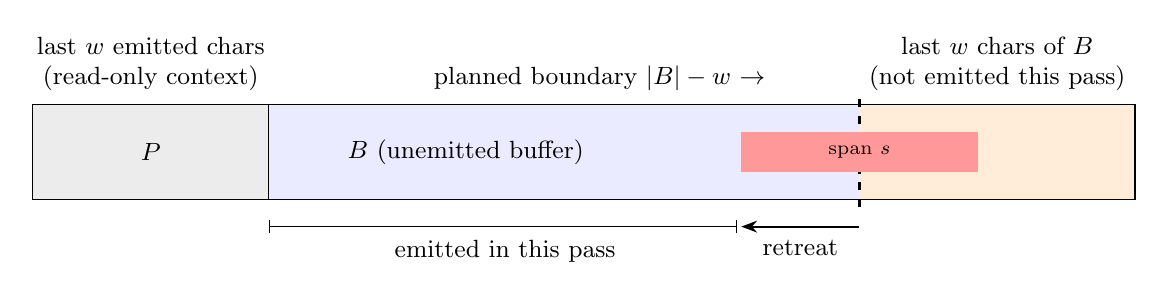
\begin{tikzpicture}[every node/.style={font=\small}]
\fill[gray!15] (0,0) rectangle (3,1.2);
\fill[blue!8] (3,0) rectangle (10.5,1.2);
\fill[orange!15] (10.5,0) rectangle (14,1.2);
\draw (0,0) rectangle (14,1.2);
\draw (3,0) -- (3,1.2);
\draw[dashed, thick] (10.5,-0.1) -- (10.5,1.3);
\node at (1.5,0.6) {$P$};
\node at (5.5,0.6) {$B$ (unemitted buffer)};
\fill[red!40] (9,0.35) rectangle (12,0.85);
\node at (10.5,0.6) {\scriptsize span $s$};
\node[above, align=center] at (1.5,1.25) {last $w$ emitted chars\\(read-only context)};
\node[above, align=center] at (12.25,1.25) {last $w$ chars of $B$\\(not emitted this pass)};
\node[above, align=center] at (7.2,1.25) {planned boundary $|B|-w$ $\rightarrow$};
\draw[-{Stealth[length=2mm]}, thick] (10.5,-0.35) -- (9,-0.35);
\node[below] at (9.75,-0.4) {retreat};
\draw[|-|] (3,-0.35) -- (8.95,-0.35);
\node[below] at (6,-0.4) {emitted in this pass};
\end{tikzpicture}}
\caption{One pass of Algorithm~\ref{alg:stream}. The detector reads $P \cdot B$; only text before the planned boundary may be emitted, and the boundary retreats out of any span that crosses it, so $s$ is carried to the next pass and detected whole.}\label{fig:window}
\end{figure}

Algorithm~\ref{alg:stream}, a simplified form of \texttt{engine.stream\_windows} illustrated in Figure~\ref{fig:window}, keeps a buffer of unemitted text and the last $w$ characters already emitted. Each pass detects over their concatenation, so detectors see real left context rather than an artificial edge, and emits only the part of the buffer that lies at least $w$ characters before its end. If a detection crosses the planned emit boundary, the boundary retreats to the detection's start and the detection is carried into the next pass. Small chunks are coalesced until at least $m$ characters can be emitted, which bounds the cost of rescanning the overlap per emitted character regardless of how the input is chunked. The defaults are $w = 8192$ characters and $m = 65{,}536$ characters.

\subsection{Parallel engine}
For large files the parallel engine splits the input into character-aligned byte ranges of at least $4w$ characters, one per worker process. Each worker reads $w$ characters of scanned padding and a further $w$ characters of context-only prefix around its interior boundaries (seams). A span that crosses a seam belongs to the left worker, and the right worker begins emitting at that span's end. Neighbouring workers compute the seam position independently, and the coordinator compares their reports; on any disagreement it discards the parallel result and redacts the file sequentially.

\subsection{Implementation}
The pure-Python implementation is the reference. An optional Rust core implements the pattern tiers. At start-up it checks that its compiled pattern sources equal the Python ones, and it hands a window back to Python in the rare cases where Unicode case folding or floating-point summation could make the two disagree.

\paragraph{Use of AI tools}
The large language model Claude (Anthropic) was used during this research to help write evaluation harness scripts, draft early versions of manuscript sections, format the \LaTeX{} source for the journal template, refine prose and check bibliographic entries. The authors independently verified all experimental outputs, mathematical proofs and manuscript text, and take full responsibility for the final work.

%% ===================================================================
\section{Formal analysis}\label{sec:formal}

Let $S_w(T)$ be the set of detections emitted by Algorithm~\ref{alg:stream} for some chunking of $T$, mapped back to absolute offsets, and $P_{w,k}(T)$ the output of the parallel engine with $k$ workers. Each detector $d \in \mathcal{D}$ declares three constants: the longest span it emits, $L_d$, and the context it reads to the left and right of a span, $C_{\mathrm{left},d}$ and $C_{\mathrm{right},d}$. The two assumptions are stated per detector and must hold for every input text, not only for $T$, because the engine applies $\Pi$ to windows.

\begin{assumption}[Bounded span]\label{as:span}
For every text $X$, every detection of detector $d$ in $\Pi(X)$ has length $j - i \le L_d$.
\end{assumption}

\begin{assumption}[Bounded context]\label{as:ctx}
Let $X$ and $Y$ be texts and $\delta$ an offset with $X[a{:}b] = Y[a{+}\delta : b{+}\delta]$. Let $(i, j)$ be a span of detector $d$ such that either $i - C_{\mathrm{left},d} \ge a$ or $a = a + \delta = 0$, and either $j + C_{\mathrm{right},d} \le b$ or both $b = |X|$ and $b + \delta = |Y|$. Then $(i, j, \tau, \kappa) \in \Pi(X)$ if and only if $(i + \delta, j + \delta, \tau, \kappa) \in \Pi(Y)$.
\end{assumption}

In words, \ref{as:ctx} says that whether a span of $d$ is in the final detection set, and with which type and confidence, depends only on the $C_{\mathrm{left},d}$ characters before it, the span itself and the $C_{\mathrm{right},d}$ characters after it, where a window edge that coincides with an edge of both texts counts as real. The pipeline requirement is
\begin{equation}\label{eq:wstar}
w^{\star} \;=\; \max_{d \in \mathcal{D}}\ \max\bigl(L_d + C_{\mathrm{right},d},\ C_{\mathrm{left},d}\bigr).
\end{equation}

\begin{theorem}[Streaming equivalence]\label{thm:stream}
Under \ref{as:span} and \ref{as:ctx}, if $w \ge w^{\star}$ and $m \ge w$, then $S_w(T) = \Pi(T)$ for every text $T$ and every chunking of $T$.
\end{theorem}

\begin{corollary}[Pipeline-wide sufficient condition]\label{cor:coarse}
Let $L_{\max} = \max_d L_d$, $C_{\mathrm{left}} = \max_d C_{\mathrm{left},d}$ and $C_{\mathrm{right}} = \max_d C_{\mathrm{right},d}$. Then $w \ge \max(L_{\max} + C_{\mathrm{right}},\, C_{\mathrm{left}})$ implies $w \ge w^{\star}$, so Theorem~\ref{thm:stream} applies.
\end{corollary}

The corollary is the intuition: the overlap must hold the longest span together with the widest right context, and the widest left context. It is sufficient but not necessary, because it pairs the longest span with a right context that may belong to a different detector. Equation~\eqref{eq:wstar} is the condition the engine checks (Section~\ref{sec:derived}).

\paragraph{Why the right context is added to the span}
An overlap of $\max_d \max(L_d, C_{\mathrm{left},d}, C_{\mathrm{right},d})$, which bounds each quantity separately, is not enough. Take a detector $d$ that rejects a candidate whose right context is missing, and an overlap $w < L_d + C_{\mathrm{right},d} - 1$. A chunking can end a pass so that a span $s = (i, j)$ of $\Pi(T)$ starts one character before the planned boundary $e_0 = |B| - w$ and has length $L_d$. Its right context then extends $(L_d - 1) + C_{\mathrm{right},d} > w$ characters beyond $e_0$, past the end of the buffer. The window therefore rejects $s$. If no other detection straddles $e_0$, the boundary does not retreat, and the pass emits $T[i : e_0]$, the first character of $s$, unredacted. A shorter span ending before $e_0$ can be emitted in its place. The bound in Eq.~\eqref{eq:wstar} is thus tight up to one character. It is also why the safe-region step in the proof below adds $C_{\mathrm{right},d}$ to $L_d$.

\begin{proof}[Proof of Theorem~\ref{thm:stream}]
Fix a non-final pass. Let $p$ be the absolute position of $B[0]$, $q = p + |B|$ and $e_0 = q - w$ the planned boundary. The window is $W = T[p - |P| : q]$, where $|P| = \min(w, p)$ because $P$ holds the last $w$ emitted characters.

\emph{Safe region.} Let $s = (i, j, \tau, \kappa)$ be a span of detector $d$, in absolute offsets, with $p \le i < e_0$ that belongs to $\Pi(W)$ or to $\Pi(T)$. By \ref{as:span}, $j \le i + L_d < q - w + L_d \le q - C_{\mathrm{right},d}$, using $w \ge L_d + C_{\mathrm{right},d}$. On the left, $i - C_{\mathrm{left},d} \ge p - w$ because $w \ge C_{\mathrm{left},d}$; if $p < w$, the window starts at position 0 of $T$. \ref{as:ctx}, applied to $X = W$ and $Y = T$, then gives $s \in \Pi(W) \Leftrightarrow s \in \Pi(T)$. So the spans of the window that start in $[p, e_0)$ are exactly the spans of $\Pi(T)$ that start there.

\emph{Retreat.} $\Pi(W)$ is pairwise disjoint, so at most one span $s^{*}$ straddles $e_0$, and it starts before $e_0$, so it belongs to $\Pi(T)$. The boundary becomes $e = i^{*}$ if $s^{*}$ exists and $e = e_0$ otherwise. In the first case, $i^{*} > e_0 - L_d \ge p + m - L_d \ge p$, because $|B| \ge w + m$ and $m \ge w \ge L_d$. So $e > p$, and the pass emits at least one character; the pinned branch is never taken. No span of $\Pi(T)$ straddles $e$. If $e = e_0$, such a span would start before $e_0$ and so be the straddler of $W$. If $e = i^{*}$, it would overlap $s^{*}$, which disjointness rules out.

\emph{Emission.} The pass emits $T[p{:}e]$ with the window spans contained in it. By the safe region these are exactly the spans of $\Pi(T)$ contained in $[p, e)$. The final pass has $q = |T|$, so the right-hand clause of \ref{as:ctx} holds for every span, and it emits exactly the spans of $\Pi(T)$ inside $[p, |T|)$. The emitted segments partition $T$, and no span of $\Pi(T)$ crosses a segment boundary. Every span of $\Pi(T)$ is therefore emitted exactly once, with the type and confidence it has in $\Pi(T)$, and nothing else is emitted.
\end{proof}

\begin{theorem}[Parallel identity with fail-safe fallback]\label{thm:par}
(i) Under the conditions of Theorem~\ref{thm:stream}, and with ranges of at least $4w$ characters, every seam report agrees and $P_{w,k}(T)$ equals the sequential output byte for byte. (ii) Without any assumption on the detectors, the output is either assembled from parts whose seam reports all agree, so that every character of $T$ is emitted exactly once, or it is the sequential output.
\end{theorem}

\begin{theorem}[Bounded working buffer]\label{thm:mem}
Let $c$ be the length of the longest input chunk. Under the conditions of Theorem~\ref{thm:stream}, the unemitted buffer of $S_w$ never exceeds $w + m + c$ characters, and each detection window never exceeds $2w + m + c$, independent of $|T|$. Each parallel worker additionally holds back at most $2w$ characters plus one segment, so the parallel engine needs $O\bigl(k\,(w + m + c)\bigr)$ characters.
\end{theorem}

Because redaction acts on each span separately (Definition~\ref{def:det}), Theorem~\ref{thm:stream} implies byte-identical redacted output. The proofs of Theorems~\ref{thm:par} and~\ref{thm:mem}, and a table mapping each step to the implementation, are in Appendix~\ref{app:proofs}. For \texttt{redact\_file}, $c = m = 65{,}536$ and $w = 8192$, so the buffer stays below 139,264 characters and each window below 147,456 characters. The proofs were not machine-checked.

\subsection{What is derived and what is assumed}\label{sec:derived}

\begin{table}[t]
\caption{Declared streaming bounds of the evaluated detectors, in characters, at the evaluated commit. The requirement of a detector is $\max(L_d + C_{\mathrm{right},d},\, C_{\mathrm{left},d})$; the pipeline requirement $w^{\star}$ is the largest requirement among active detectors.}\label{tab:bounds}
\footnotesize
\begin{tabular*}{\textwidth}{@{\extracolsep\fill}lrrrr}
\toprule
Detector $d$ & $L_d$ & $C_{\mathrm{left},d}$ & $C_{\mathrm{right},d}$ & Requirement \\
\midrule
Deterministic patterns & 8192 & 0 & 0 & 8192 \\
Label-anchored identifiers & 64 & 96 & 8 & 96 \\
Entropy tier & 8192 & 32 & 0 & 8192 \\
Compound entropy tier & 8192 & 0 & 0 & 8192 \\
Contextual scorer & 9 & 48 & 0 & 48 \\
spaCy named-entity tier (optional) & 256 & 256 & 256 & 512 \\
\midrule
Default pipeline, $w^{\star}$ & & & & 8192 \\
Default pipeline with spaCy, $w^{\star}$ & & & & 8192 \\
\bottomrule
\end{tabular*}
\end{table}

Each detector declares $(L_d, C_{\mathrm{left},d}, C_{\mathrm{right},d})$. The engine computes $w^{\star}$ from Eq.~\eqref{eq:wstar} over the active detectors and refuses to start with a smaller overlap unless the caller explicitly overrides it. Table~\ref{tab:bounds} lists the declarations. The detectors that emit the longest spans (private-key blocks and entropy candidates, $L_d = 8192$) read no right context. The only detector with right context among the default tiers, the label-anchored tier, emits spans of at most 64 characters. Hence $w^{\star} = 8192$, and the default overlap $w = 8192$ satisfies Theorem~\ref{thm:stream} exactly, with or without the spaCy tier. The pipeline-wide Corollary~\ref{cor:coarse} would ask for $8192 + 8 = 8200$ characters; that is why the per-detector form is the one the engine enforces. A regression test fails if any declaration changes, and a differential test probes each detector to check that its real context dependency does not exceed its declaration.

Two parts of \ref{as:span} and \ref{as:ctx} are \emph{not} derived from declarations. They should be read as assumptions corroborated by tests rather than proven properties of the code. (i) The confidence adjustment and threshold must not reach beyond the declared context of the detector whose span they adjust. The contextual scorer's 48-character left window is within $w$ for every detector, but it is not added to the other detectors' declarations. (ii) Overlap resolution must not propagate decisions along chains of overlapping candidates beyond the declared contexts, and the named-entity union rule must not create spans longer than the declared bounds. For the pattern tiers, whose spans are bounded and whose overlaps are short, the equivalence tests in Section~\ref{sec:equiv} found no counterexample. A statistical model's output can depend on its whole input window, so for the spaCy tier the declared bounds of 256 characters are declarations only, and the theorems should not be read as covering it. Empirically, its streamed output matched the whole-document output in every chunking we tried (Section~\ref{sec:equiv}).

\paragraph{Failure modes}
Lowering the overlap below $w^{\star}$ is refused by default. If a caller overrides that, the parallel engine still cannot lose or duplicate characters (Theorem~\ref{thm:par}(ii)), but the sequential engine can split a long span. A detector that understates its context, or one that needs document-wide context, is outside the guarantee.

%% ===================================================================
\section{Experimental methodology}\label{sec:setup}

The evaluation addresses five questions. \textbf{RQ1}: do the implementation's streamed, parallel and native outputs match the reference in practice, and how often does chunking without the guarantee leak? \textbf{RQ2}: how do memory and throughput scale? \textbf{RQ3}: how well do the pattern tiers detect credentials compared with purpose-built scanners? \textbf{RQ4}: how well does SafeStream detect personal data compared with Presidio, with and without a named-entity model? \textbf{RQ5}: how much protection does it give at the level of a whole document, and how much of that depends on rules written after seeing the benchmark?

\subsection{Corpora and splits}
Table~\ref{tab:corpora} lists the test splits. Each corpus was split once into development and test halves with a fixed seed. The manifests list document identifiers and the SHA-256 of the source data, and the loader refuses a source that no longer matches. Development, error analysis and tuning used development halves only, with the exception of RedactionBench described below; test halves were scored after the code was frozen, with one disclosed exception (Section~\ref{sec:fp}).
\begin{itemize}
\item \textbf{presidio-research} \cite{presidioresearch} (synthetic): the dataset distributed with Presidio's evaluation toolkit (revision 0cb3650), with person, location, organisation, telephone, card, date and other labels, generated from templates. The 750 test documents come from 200 templates (median 3.5 documents per template).
\item \textbf{secrets} (semi-synthetic): the labelled examples in the Nosey Parker rule set \cite{noseyparker} (revision 2e6e7f3) as positives, with gold spans given by each rule's own capture groups, plus 200 generated non-secrets (UUIDs, commit hashes, SHA-256 digests, base64 image payloads, minified JavaScript) as gold-free documents. The split is by rule, so the test half contains vendor formats absent from the development half; its 216 positives come from 96 rules. The positives are short examples written by rule authors, not credentials observed in real artefacts.
\item \textbf{RedactionBench} \cite{brynjolfsson2026redactionbench}: 200 documents across eleven domains, a majority seeded from real-world sources according to its authors, with character spans labelled \emph{mandatory} or \emph{contextual}. The test half holds between 5 and 17 documents per domain. All 200 documents were used for error analysis and rule writing before the split existed, so its test half is not held out (Section~\ref{sec:contam}).
\end{itemize}

\begin{table}[t]
\caption{Test splits. Gold-free documents contain no gold span; any detection on them is a false alarm. Clusters are the resampling units of the cluster and two-stage bootstrap (Section~\ref{sec:stats}).}\label{tab:corpora}
\footnotesize
\begin{tabular*}{\textwidth}{@{\extracolsep\fill}lrrrrl}
\toprule
Corpus & Documents & Gold spans & Gold-free & Bytes & Clusters \\
\midrule
presidio-research & 750 & 1,394 & 63 & 63,678 & 200 templates \\
secrets & 313 & 293 & 97 & 46,595 & 96 rules + 5 templates \\
RedactionBench & 100 & 25,592 & 0 & 1,378,267 & 11 domains \\
\bottomrule
\end{tabular*}
\end{table}

\subsection{Systems and configurations}
\textbf{SafeStream} was run with the Rust core and default tiers (\emph{pattern}), with the opt-in date tier (\emph{+dates}), and with the spaCy \texttt{en\_core\_web\_sm} tier (\emph{+spaCy}). \textbf{Presidio} 2.2.355 \cite{presidio} was run as its pattern recognisers alone (\emph{regex}) and as the full analyser with spaCy \texttt{en\_core\_web\_sm} (\emph{sm}) and \texttt{en\_core\_web\_lg} (\emph{lg}), with spaCy 3.8.13 and models 3.8.0. \textbf{gitleaks} 8.28.0 \cite{gitleaks} and \textbf{TruffleHog} 3.90.8 \cite{trufflehog} were run with default rules and default false-positive filtering; TruffleHog ran with \texttt{--no-verification}, so no example credential was sent to a live service. A sensitivity run repeated both scanners with their false-positive filters disabled (Section~\ref{sec:sens}). Each scanner ran once over a directory with one file per document, and findings were mapped back to character offsets; TruffleHog's composite findings (for example \texttt{user:token}) were credited for each component that appears in the text. Presidio received documents longer than 20,000 characters in line-aligned pieces of at most that length; no gold span in any test split crosses a piece boundary, so the splitting cost Presidio no recall. Each Python tool ran in its own virtual environment and process, pinned to one thread; the scanners are Go binaries and ran with their default concurrency. All SafeStream thresholds are defaults; no threshold was tuned on test data. The RedactionBench dev-selected configurations (Section~\ref{sec:contam}) were chosen on the development half by a rule fixed in advance.

\subsection{Metrics}
Let $G$ and $R$ be the sets of gold and redacted character positions in a document. Character precision and recall are $|G \cap R| / |R|$ and $|G \cap R| / |G|$, summed over documents, and F1 is their harmonic mean. All metrics are type-agnostic: a value counts as protected whatever label it receives. The \emph{fully redacted rate} is the share of gold spans with every character redacted. The \emph{false-alarm document rate} is the share of gold-free documents with at least one detection. On RedactionBench, \emph{mandatory recall} is character recall over mandatory spans, and the \emph{no-leak document rate} is the share of documents in which every mandatory character is redacted (Section~\ref{sec:noleak} discusses how it relates to recall).

\subsection{Statistical analysis}\label{sec:stats}
We report 95\% percentile bootstrap intervals with 2,000 resamples and seed 0 \cite{efron1993bootstrap}. All systems evaluated on a corpus are scored on one shared resample matrix, so every difference between two systems is paired; we report the median paired difference and call it significant only when its paired interval excludes zero. Documents are not independent. Secrets positives cluster by rule, presidio-research documents share generator templates, and RedactionBench documents share domains. We therefore use three resampling schemes on the same per-document counts \cite{field2007bootstrapping}: \emph{document} (documents drawn independently), \emph{cluster} (whole clusters drawn with replacement, all their documents kept) and \emph{two-stage} (clusters drawn with replacement, then documents drawn with replacement inside each drawn cluster). Table~\ref{tab:corpora} lists the clusters. Tables~\ref{tab:main}, \ref{tab:rb} and~\ref{tab:ablation} give document-level intervals. Table~\ref{tab:cluster} repeats the planned comparisons under all three schemes, and we call a difference \emph{robust} when it is significant under all three. RedactionBench has only eleven clusters, so its cluster intervals are themselves imprecise; we read them as a sensitivity analysis rather than as an exact test. No correction for multiple comparisons was applied; the comparisons in the abstract were planned, the ablation comparisons were not. The analysis was not pre-registered.

\subsection{Environment}
Accuracy runs used a 4-vCPU Intel Xeon virtual machine at 2.80\,GHz with 15\,GB RAM, Linux and CPython 3.13. Throughput figures come from separate runs, five per configuration, on the same machine with no other benchmark running; the throughput recorded during accuracy runs is not used. Memory was measured as the peak resident set size of a fresh process per point minus its resident set size after imports, so native allocations are included; it is reported in MiB. The cluster analysis re-ran every test-split system at the evaluated commits with the same tool versions and saved per-document predictions; each point estimate and each document-level paired interval reproduced the published values to three decimals. The held-out results come from commit \texttt{0765dae}, the results after the entropy fix (Section~\ref{sec:fp}) from \texttt{3d2c6ac}, and the pre-exposure RedactionBench results from \texttt{874e105}, all on the main branch of the public repository.

%% ===================================================================
\section{Results}\label{sec:results}

\subsection{RQ1: equivalence, backend parity and leaks caused by chunking}\label{sec:equiv}
On every test split the Rust core and the pure-Python reference produced identical predictions (presidio-research 178 spans, secrets 298, RedactionBench 3,167, from the frozen commit). The repository's equivalence suite asserts byte-identical streamed, whole-document and parallel output over exhaustive small chunkings, property-based generated inputs, seam-straddling entities and forced fallbacks, and also checks native parity and declared context; it passed 133 of 133 tests at the final commit. These tests corroborate the theorems for the configurations they exercise; they are not proofs, and they do not exercise the named-entity tier's full input dependence.

\paragraph{How often chunking alone leaks}
The theorems say that chunking cannot add leaks; they do not say how many leaks chunking adds without them. To measure that, we concatenated each test split into one stream, two newlines between documents, and ran the same pattern pipeline in four ways (Table~\ref{tab:chunk}; script \texttt{benchmarks/chunking\_leak.py}):
\begin{itemize}
\item \emph{whole}: one pass over the stream, the reference $\Pi(T)$;
\item \emph{naive}: fixed chunks of $c$ characters, each detected on its own;
\item \emph{overlapping windows}: windows of $c + o$ characters advancing by $c$, each keeping the detections that start in its own $c$ characters, which is common practice; we used $o = 256$ and $o = 8192$, the longest declared span;
\item \emph{SafeStream}: Algorithm~\ref{alg:stream} at its default overlap and the smallest allowed emit size ($m = w$), on five random chunkings per chunk size with chunk lengths drawn uniformly from $1$ to $2c$.
\end{itemize}
We also ran a 4.2\,MB log produced by the repository's generator, with 56,153 gold values, as a stand-in for a dense machine log.

Naive chunking leaked gold values that the whole-document pass redacts on every corpus. At $c$ = 1\,KiB it leaked 237 RedactionBench values, 7 on presidio-research and 5 on secrets, and 872 values in the generated log; at 64\,KiB it still leaked 1 RedactionBench value and 12 in the log. A leaked value can be part of a larger gold region, so the number of leaked gold spans can exceed the number of missed detections. Overlapping windows removed most of these leaks, but not all. At 1\,KiB they still missed 3 RedactionBench detections and leaked 2 RedactionBench values, 1 presidio-research value and 2 secrets, even with $o = 8192$. In the pattern runs with $o = 8192$, all seven residual misses start 5 to 9 characters into their window and come from detectors that read a cue to their left (a key name, a URL-credential prefix, an account label). The cue lay in the previous window, which these windows discard, so a longer overlap $o$, which only extends a window to the right, cannot recover them. SafeStream keeps exactly this context as its read-only prefix $P$. Both naive and overlapping chunking also redacted characters the whole-document pass does not (up to 2,738 in the log), from candidates cut short at a window edge. SafeStream's detection set was identical to the whole-document reference in all 80 pattern-tier runs: four corpora, four chunk sizes and five chunkings each. The same held with the spaCy tier on presidio-research and on the first 66 RedactionBench test documents (928,652 characters, below spaCy's 1,000,000-character input limit), at 4\,KiB and 64\,KiB with two chunkings each. That last result is an empirical check, not a proof, because the theorems do not cover the spaCy tier (Section~\ref{sec:derived}).

\begin{table}[t]
\caption{Leaks caused by chunking alone. Each cell gives missed reference detections / gold spans leaked by chunking (fully redacted by the whole-document pass, not by the variant). SafeStream: runs whose detection set is identical to the whole-document reference, out of the random chunkings tried. Overlapping windows keep the detections that start in their own chunk; $o$ is the window overlap in characters. The generated log is synthetic and dense (56,153 gold values in 4.2\,MB).}\label{tab:chunk}
\footnotesize
\setlength{\tabcolsep}{3pt}
\begin{tabular*}{\textwidth}{@{\extracolsep\fill}llrrrl}
\toprule
Corpus (pipeline) & Chunk $c$ & Naive & $o = 256$ & $o = 8192$ & SafeStream \\
\midrule
secrets (pattern) & 1\,KiB & 11 / 5 & 4 / 3 & 2 / 2 & 5 of 5 \\
 & 4\,KiB & 3 / 1 & 1 / 1 & 0 / 0 & 5 of 5 \\
 & 64\,KiB & 0 / 0 & 0 / 0 & 0 / 0 & 5 of 5 \\
presidio-research (pattern) & 1\,KiB & 5 / 7 & 1 / 1 & 1 / 1 & 5 of 5 \\
 & 4\,KiB & 0 / 0 & 0 / 0 & 0 / 0 & 5 of 5 \\
 & 64\,KiB & 0 / 0 & 0 / 0 & 0 / 0 & 5 of 5 \\
RedactionBench (pattern) & 1\,KiB & 74 / 237 & 3 / 2 & 3 / 2 & 5 of 5 \\
 & 4\,KiB & 9 / 10 & 1 / 0 & 1 / 0 & 5 of 5 \\
 & 64\,KiB & 1 / 1 & 0 / 0 & 0 / 0 & 5 of 5 \\
Generated log (pattern) & 1\,KiB & 957 / 872 & 0 / 0 & 0 / 0 & 5 of 5 \\
 & 4\,KiB & 234 / 212 & 0 / 0 & 0 / 0 & 5 of 5 \\
 & 64\,KiB & 16 / 12 & 0 / 0 & 0 / 0 & 5 of 5 \\
presidio-research (+spaCy) & 4\,KiB & 2 / 1 & 0 / 0 & 0 / 0 & 2 of 2 \\
 & 64\,KiB & 0 / 0 & 0 / 0 & 0 / 0 & 2 of 2 \\
RedactionBench, 66 docs (+spaCy) & 4\,KiB & 20 / 10 & 2 / 0 & 2 / 0 & 2 of 2 \\
 & 64\,KiB & 0 / 0 & 0 / 0 & 0 / 0 & 2 of 2 \\
\bottomrule
\end{tabular*}
\footnotetext{The 16\,KiB rows are in the result files (\texttt{research/results/raw/2026-11-12\_chunking\_leak\_*.json}); they fall between the 4\,KiB and 64\,KiB rows.}
\end{table}

\subsection{RQ2: memory and throughput}\label{sec:memory}

\begin{figure}[t]
\centering
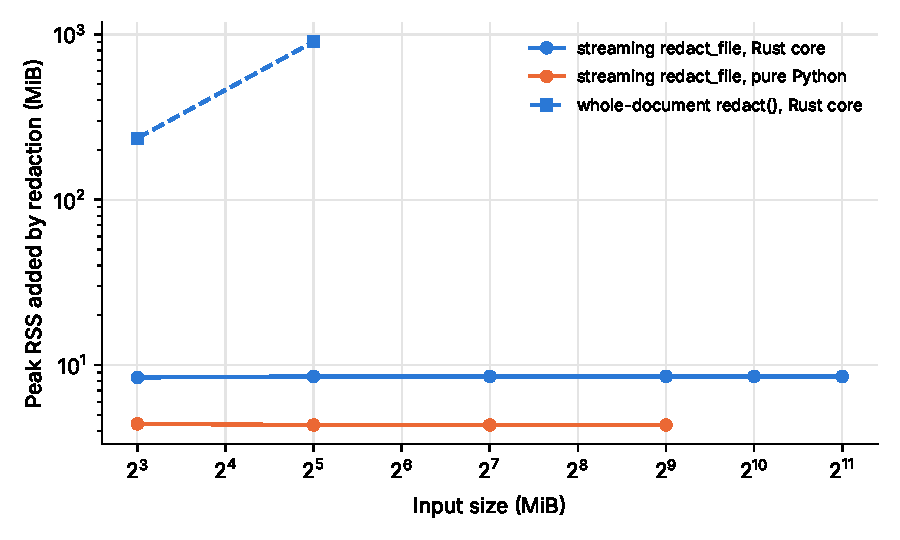
\includegraphics[width=0.85\textwidth]{fig_memory.pdf}
\caption{Peak resident memory added by redaction (peak RSS minus RSS after imports, MiB) against input size, log scales, each point a fresh process. Streaming \texttt{redact\_file} stays flat from 8\,MiB to 2\,GiB (Rust core) and to 512\,MiB (pure Python); whole-document \texttt{redact()} grows with the input.}\label{fig:memory}
\end{figure}

Figure~\ref{fig:memory} plots peak resident memory against input size. Each point is a fresh process redacting a generated log file dense with personal data and credentials. With the Rust core, streaming \texttt{redact\_file} added between 8.4 and 8.54\,MiB at every size from 8\,MiB to 2\,GiB, a 256-fold range. The pure-Python backend added between 4.3 and 4.4\,MiB from 8 to 512\,MiB; it was not run at larger sizes because of its run time (726\,s at 512\,MiB). Whole-document \texttt{redact()} on the same generated inputs, measured the same way, added 235.5\,MiB at 8\,MiB and 904.6\,MiB at 32\,MiB, about 28 times the input size, because the input string, the detections and the output are held at once; at 32\,MiB the two modes therefore differ by a factor of about 106 on identical input. A 128\,MiB whole-document run was stopped after 20 minutes without completing and is not reported. These measurements are consistent with Theorem~\ref{thm:mem} but cover one generated input shape on one machine, and only two whole-document sizes.

\begin{table}[t]
\caption{Throughput on the test splits in MB/s, mean $\pm$ sample standard deviation over 5 runs, one thread, load time excluded. Each run is a fresh process on an otherwise idle 4-vCPU machine.}\label{tab:throughput}
\footnotesize
\begin{tabular*}{\textwidth}{@{\extracolsep\fill}llll}
\toprule
System & presidio-research & secrets & RedactionBench \\
\midrule
SafeStream pattern (Rust core) & $1.82 \pm 0.42$ & $2.39 \pm 0.58$ & $10.4 \pm 1.3$ \\
SafeStream pattern (pure Python) & $1.10 \pm 0.07$ & $0.916 \pm 0.17$ & $1.23 \pm 0.15$ \\
SafeStream +spaCy (sm) & $0.0118 \pm 0.0009$ & $0.0227 \pm 0.0034$ & $0.0467 \pm 0.0033$ \\
Presidio regex & $0.0802 \pm 0.0127$ & $0.0983 \pm 0.0155$ & $0.0694 \pm 0.0028$ \\
Presidio sm & $0.0081 \pm 0.0004$ & $0.0125 \pm 0.0007$ & $0.0201 \pm 0.0003$ \\
Presidio lg & $0.0074 \pm 0.0010$ & $0.0128 \pm 0.0008$ & $0.0203 \pm 0.0003$ \\
gitleaks\footnotemark[1] & $0.507 \pm 0.028$ & $0.409 \pm 0.051$ & $3.15 \pm 0.19$ \\
TruffleHog\footnotemark[1] & $0.0269 \pm 0.0016$ & $0.0188 \pm 0.0007$ & $0.594 \pm 0.020$ \\
\bottomrule
\end{tabular*}
\footnotetext[1]{Go binaries run once per corpus over a directory of documents; the figure includes process start-up and is not limited to one thread.}
\end{table}

Table~\ref{tab:throughput} reports throughput on the test splits. Per-document overhead dominates on presidio-research and secrets, whose documents average 85 and 149 bytes; RedactionBench's documents average 13.8\,kB. There the Rust core processed $10.4 \pm 1.3$\,MB/s, the pure-Python reference $1.23 \pm 0.15$\,MB/s and Presidio's pattern recognisers 0.069\,MB/s. With a statistical model in the loop every system ran below 0.05\,MB/s: SafeStream +spaCy at 0.047\,MB/s and Presidio sm and lg at 0.020\,MB/s. The scanner figures include process start-up and are not comparable per thread.

\begin{figure}[t]
\centering
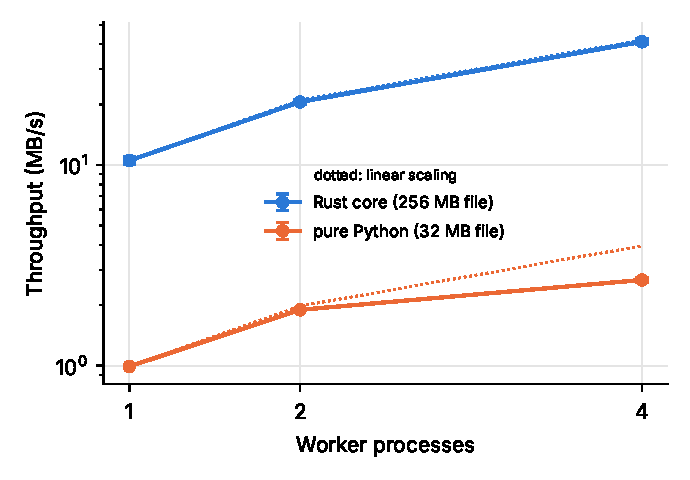
\includegraphics[width=0.62\textwidth]{fig_scaling.pdf}
\caption{Throughput of \texttt{redact\_file} against worker processes on a 4-vCPU machine, mean and standard deviation over 5 runs (log scale). Dotted lines show linear scaling from one worker. The parallel output is byte-identical to the sequential output (Theorem~\ref{thm:par}).}\label{fig:scaling}
\end{figure}

On a single 256\,MB generated log file (mostly benign log lines and prose with personal data and credentials mixed in), \texttt{redact\_file} with the Rust core ran at $10.5 \pm 0.5$, $20.6 \pm 0.5$ and $41.1 \pm 1.4$\,MB/s with 1, 2 and 4 worker processes, a 3.9-fold speed-up on 4 vCPUs (Figure~\ref{fig:scaling}). The pure-Python backend on a 32\,MB file of the same kind ran at 0.99, 1.90 and 2.67\,MB/s. These figures come from one virtual machine and should be read as relative rather than absolute.

\subsection{RQ3 and RQ4: detection on held-out data}

\begin{figure}[t]
\centering
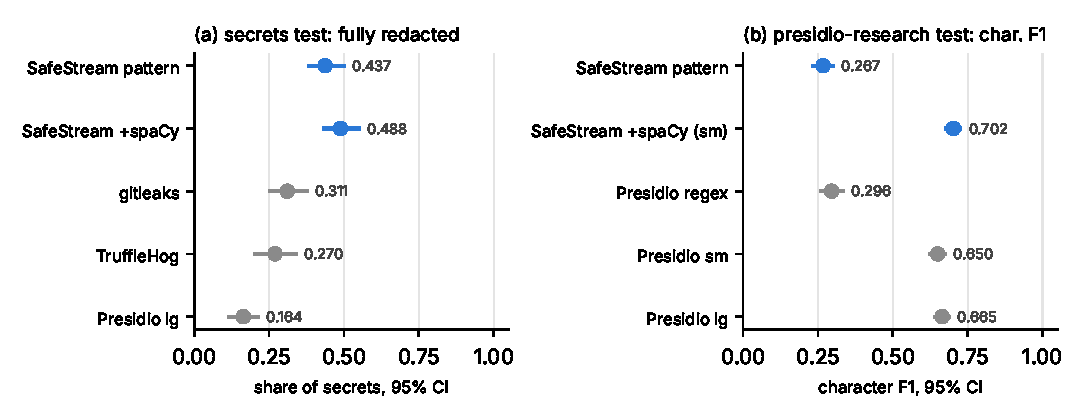
\includegraphics[width=\textwidth]{fig_accuracy.pdf}
\caption{Test-split accuracy with 95\% document-level bootstrap intervals. (a) Share of secrets fully redacted on the secrets test split. (b) Character F1 on the presidio-research test split. SafeStream configurations in blue, baselines in grey.}\label{fig:accuracy}
\end{figure}

\begin{table}[t]
\caption{Test-split results with 95\% document-level bootstrap intervals. SafeStream rows are after the entropy fix of Section~\ref{sec:fp}, which changed only the secrets results. FR: fully redacted rate; FA: false-alarm document rate.}\label{tab:main}
\footnotesize
\setlength{\tabcolsep}{3pt}
\begin{tabular*}{\textwidth}{@{\extracolsep\fill}llllll}
\toprule
Corpus / system & Char P & Char R & Char F1 & FR & FA \\
\midrule
\multicolumn{6}{@{}l}{\emph{presidio-research (750 documents)}}\\
SafeStream pattern & \pc{.995}{.992, .998} & \pc{.154}{.133, .176} & \pc{.267}{.235, .299} & \pc{.115}{.098, .134} & .000 \\
SafeStream +dates & \pc{.996}{.993, .998} & \pc{.169}{.146, .192} & \pc{.290}{.255, .322} & \pc{.129}{.110, .150} & .000 \\
SafeStream +spaCy (sm) & \pc{.898}{.877, .918} & \pc{.576}{.547, .606} & \pc{.702}{.679, .725} & \pc{.538}{.509, .568} & .079 \\
Presidio regex & \pc{.948}{.919, .974} & \pc{.175}{.151, .202} & \pc{.296}{.260, .333} & \pc{.123}{.105, .145} & .000 \\
Presidio sm & \pc{.871}{.848, .893} & \pc{.518}{.491, .546} & \pc{.650}{.626, .673} & \pc{.506}{.479, .536} & .048 \\
Presidio lg & \pc{.878}{.856, .900} & \pc{.535}{.507, .563} & \pc{.665}{.642, .688} & \pc{.562}{.534, .590} & .000 \\
\midrule
\multicolumn{6}{@{}l}{\emph{secrets (313 documents)}}\\
SafeStream pattern & \pc{.857}{.705, .946} & \pc{.829}{.740, .887} & \pc{.842}{.736, .906} & \pc{.437}{.384, .498} & .010 \\
SafeStream +spaCy (sm) & \pc{.757}{.604, .858} & \pc{.845}{.762, .897} & \pc{.799}{.683, .870} & \pc{.488}{.435, .548} & .340 \\
gitleaks & \pc{.837}{.630, .962} & \pc{.473}{.299, .679} & \pc{.604}{.430, .765} & \pc{.311}{.253, .375} & .000 \\
TruffleHog & \pc{.803}{.719, .878} & \pc{.189}{.117, .308} & \pc{.306}{.204, .446} & \pc{.270}{.204, .340} & .000 \\
Presidio regex & \pc{.282}{.211, .356} & \pc{.105}{.063, .177} & \pc{.153}{.098, .225} & \pc{.126}{.083, .168} & .392 \\
Presidio sm & \pc{.251}{.191, .315} & \pc{.119}{.072, .197} & \pc{.161}{.107, .232} & \pc{.160}{.112, .206} & .649 \\
Presidio lg & \pc{.308}{.238, .381} & \pc{.131}{.082, .214} & \pc{.184}{.124, .262} & \pc{.164}{.116, .212} & .433 \\
\bottomrule
\end{tabular*}
\end{table}

Table~\ref{tab:main} and Figure~\ref{fig:accuracy} give the test-split results; Table~\ref{tab:cluster} tests the planned differences under clustering.

\paragraph{Credentials (RQ3)}
On secrets, SafeStream's pattern tiers fully redacted 0.437 of test secrets, against 0.311 for gitleaks and 0.270 for TruffleHog. With documents resampled independently, the paired differences in fully redacted rate were $+0.128$ [$+0.073$, $+0.183$] and $+0.167$ [$+0.079$, $+0.250$], and in character F1 $+0.233$ [$+0.043$, $+0.441$] and $+0.536$ [$+0.310$, $+0.685$]. The differences in character precision were not significant ($+0.005$ [$-0.063$, $+0.123$] and $+0.060$ [$-0.109$, $+0.176$]). Resampling by rule widens every interval (Table~\ref{tab:cluster}). The advantage over gitleaks remains significant in both fully redacted rate (two-stage $+0.125$ [$+0.025$, $+0.209$]) and character F1 ($+0.226$ [$+0.011$, $+0.538$]). Against TruffleHog the character-F1 advantage remains ($+0.530$ [$+0.192$, $+0.742$]), but the fully-redacted-rate advantage does not ($+0.184$ [$-0.008$, $+0.363$]); that margin is not robust to dependence between examples of the same rule. SafeStream flagged one of 97 generated non-secrets; neither scanner flagged any. More than half of the test secrets (0.563) were not fully redacted by SafeStream either. The development recall (0.542) exceeded the test recall (0.437) because the test half holds vendor formats for which SafeStream has no pattern. Presidio has no credential recognisers, and adding spaCy raised SafeStream's false-alarm rate to 0.340; on the development split those false alarms were the word \texttt{Merge} in commit lines tagged as a person and digest or UUID tokens tagged as persons or organisations.

\paragraph{Scanner sensitivity}\label{sec:sens}
The gold labels are Nosey Parker's rule examples, and both scanners apply false-positive filters designed to suppress example- or placeholder-like strings, so their default configurations may be penalised more than they would be on real data. We therefore re-ran both scanners with these filters disabled (Table~\ref{tab:sens}). For gitleaks we removed the global allowlist and all nine per-rule allowlists, which hold its stopwords, from the release's own configuration file, leaving all 217 rules (regexes, keywords and entropy thresholds) unchanged; the unmodified file reproduced the built-in default exactly. For TruffleHog we added the results its false-positive filter drops (\texttt{--results} including \texttt{filtered\_unverified}), still without verification. Both filters-off runs are supersets of the defaults. gitleaks gained substantially in character recall (0.473 to 0.737) and F1 (0.604 to 0.805) but little in fully redacted rate (0.311 to 0.328): its filters suppressed few findings, in 6 of 313 documents, but long ones. Against filters-off gitleaks, SafeStream's fully-redacted-rate advantage remains robust ($+0.111$ [$+0.058$, $+0.163$]; two-stage $+0.106$ [$+0.008$, $+0.193$]), whereas its character-F1 advantage shrinks to $+0.039$ [$+0.008$, $+0.093$] and does not survive rule clustering ($+0.039$ [$-0.007$, $+0.141$]). TruffleHog changed little (fully redacted 0.270 to 0.290, F1 0.306 to 0.314), and the conclusions against it are unchanged: the F1 advantage is robust and the fully-redacted-rate advantage is not. On RedactionBench, disabling the filters raised gitleaks' mandatory recall from 0.247 to 0.284 and left TruffleHog essentially unchanged; pre-exposure SafeStream exceeded both filters-off scanners in character F1 and mandatory recall under all three schemes. SafeStream's own credential patterns were not developed on the secrets corpus: it was added after the split was fixed, and the only change made using it was the suppression rule of Section~\ref{sec:fp}, designed on the development half.

\begin{table}[t]
\caption{Secret scanners on the secrets test split with default false-positive filters and with the filters disabled, with 95\% document-level intervals, and SafeStream's pattern tiers minus each scanner (paired, two-stage rule-clustered bootstrap). FR: fully redacted rate. \ns\ marks an interval that includes zero.}\label{tab:sens}
\footnotesize
\setlength{\tabcolsep}{3pt}
\begin{tabular*}{\textwidth}{@{\extracolsep\fill}llllll}
\toprule
Scanner & Filters & Char F1 & FR & SafeStream $-$ scanner, F1 & SafeStream $-$ scanner, FR \\
\midrule
gitleaks & default & \pc{.604}{.430, .765} & \pc{.311}{.253, .375} & \pc{$+.226$}{$+.011$, $+.538$} & \pc{$+.125$}{$+.025$, $+.209$} \\
gitleaks & disabled & \pc{.805}{.664, .885} & \pc{.328}{.269, .394} & \pc{$+.039$\ns}{$-.007$, $+.141$} & \pc{$+.106$}{$+.008$, $+.193$} \\
TruffleHog & default & \pc{.306}{.204, .446} & \pc{.270}{.204, .340} & \pc{$+.530$}{$+.192$, $+.742$} & \pc{$+.184$\ns}{$-.008$, $+.363$} \\
TruffleHog & disabled & \pc{.314}{.211, .454} & \pc{.290}{.225, .363} & \pc{$+.522$}{$+.182$, $+.737$} & \pc{$+.163$\ns}{$-.028$, $+.358$} \\
\bottomrule
\end{tabular*}
\end{table}

\paragraph{Personal data (RQ4)}
On presidio-research, the pattern tiers were precise (character precision 0.995) but recalled only 0.154 of sensitive characters, because most gold spans are names, locations and organisations that patterns cannot capture. Against Presidio's pattern recognisers, the paired difference in character recall was $-0.021$ [$-0.041$, $-0.002$] and in precision $+0.047$ [$+0.021$, $+0.076$]; under template clustering the precision advantage remains ($+0.046$ [$+0.011$, $+0.103$]) and the recall deficit is no longer significant. With the same spaCy model, SafeStream +spaCy exceeded Presidio sm in character F1 by $+0.051$ [$+0.027$, $+0.076$] and in fully redacted rate by $+0.031$ [$+0.004$, $+0.060$]. The F1 advantage is robust to template clustering (two-stage $+0.052$ [$+0.013$, $+0.093$]); the fully-redacted-rate advantage is not ($+0.033$ [$-0.014$, $+0.080$]). Against Presidio lg, which uses a larger model, SafeStream +spaCy had higher character F1 with documents resampled independently ($+0.036$ [$+0.011$, $+0.064$]), but not under template clustering ($+0.037$ [$-0.003$, $+0.080$]). The difference in fully redacted rate, $-0.025$ [$-0.053$, $+0.004$], was not significant under any scheme. This corpus is synthetic and template-generated; the comparison shows relative behaviour on that distribution only.

\subsection{False alarms on high-entropy non-secrets}\label{sec:fp}

Before the fix described in Section~\ref{sec:tiers}, SafeStream flagged 83 of the 103 generated non-secrets in the development split (false-alarm rate 0.806), all through the entropy tier: every UUID, commit hash, SHA-256 digest and base64 image payload, and none of the minified JavaScript. The suppression rule was designed on the development split. A first version cost one development secret, a UUID-shaped access key assigned to \texttt{SAUCE\_ACCESS\_KEY}, which led to the secret-key veto. With the veto, the development false-alarm rate fell to 0.000 with no change in recall, and the presidio-research and RedactionBench development results were unchanged except in the fourth decimal. On the test split, the false-alarm rate fell from 0.794 [0.714, 0.872] to 0.010 [0.000, 0.035], character precision rose from 0.589 to 0.857, and recall was unchanged (0.829 character recall, 0.437 fully redacted). The test half had been scored once with the pre-fix code before the fix was made; both scores are reported. Because the gold-free documents in both halves come from the same generator, the test improvement is an optimistic estimate of the fix's effect on real non-secrets.

\subsection{RQ5: document-level protection and contamination}\label{sec:contam}

\begin{table}[t]
\caption{RedactionBench test half (100 documents), with 95\% document-level bootstrap intervals. \emph{Exposed}: current code, whose rules were written after inspecting all 200 documents. \emph{Pre-exposure}: the last commit before the benchmark entered the repository. \emph{Dev-selected}: configuration chosen on the development half by a fixed rule (maximum development character F1) and scored on the test half once.}\label{tab:rb}
\footnotesize
\begin{tabular*}{\textwidth}{@{\extracolsep\fill}llll}
\toprule
System & Char F1 & Mandatory recall & No-leak docs \\
\midrule
Pre-exposure, pattern & .518 [.434, .593] & .589 [.476, .696] & .074 [.022, .129] \\
Pre-exposure, +spaCy & .472 [.395, .547] & .674 [.566, .779] & .137 [.073, .208] \\
Pre-exposure, dev-selected & .469 [.394, .543] & .676 [.568, .781] & .137 [.073, .208] \\
Exposed, pattern & .579 [.490, .662] & .682 [.578, .787] & .084 [.032, .144] \\
Exposed, +spaCy & .512 [.429, .590] & .761 [.657, .860] & .179 [.105, .263] \\
Exposed, dev-selected & .508 [.427, .588] & .762 [.658, .862] & .179 [.105, .263] \\
\midrule
gitleaks & .214 [.130, .314] & .247 [.140, .372] & .021 [.000, .053] \\
TruffleHog & .030 [.017, .048] & .024 [.013, .040] & .000 \\
Presidio regex & .323 [.250, .393] & .331 [.227, .422] & .011 [.000, .033] \\
Presidio sm & .336 [.265, .402] & .416 [.326, .500] & .084 [.032, .146] \\
Presidio lg & .344 [.277, .409] & .420 [.333, .499] & .105 [.052, .174] \\
\bottomrule
\end{tabular*}
\end{table}

\begin{table}[t]
\caption{Planned paired comparisons under three bootstrap schemes: median paired difference and 95\% interval (2,000 resamples, seed 0, one shared resample matrix per corpus). \ns\ marks an interval that includes zero. Pre-exposure SafeStream on RedactionBench is compared with every baseline because it never saw the benchmark.}\label{tab:cluster}
\footnotesize
\setlength{\tabcolsep}{3pt}
\begin{tabular*}{\textwidth}{@{\extracolsep\fill}lllll}
\toprule
Comparison & Metric & Document & Cluster & Two-stage \\
\midrule
\multicolumn{5}{@{}l}{\emph{secrets: clusters are 96 rules and 5 negative templates}}\\
Pattern $-$ gitleaks & FR & \pc{$+.128$}{$+.073$, $+.183$} & \pc{$+.123$}{$+.033$, $+.206$} & \pc{$+.125$}{$+.025$, $+.209$} \\
Pattern $-$ gitleaks & Char F1 & \pc{$+.233$}{$+.043$, $+.441$} & \pc{$+.215$}{$+.013$, $+.527$} & \pc{$+.226$}{$+.011$, $+.538$} \\
Pattern $-$ TruffleHog & FR & \pc{$+.167$}{$+.079$, $+.250$} & \pc{$+.178$\ns}{$-.010$, $+.350$} & \pc{$+.184$\ns}{$-.008$, $+.363$} \\
Pattern $-$ TruffleHog & Char F1 & \pc{$+.536$}{$+.310$, $+.685$} & \pc{$+.529$}{$+.192$, $+.740$} & \pc{$+.530$}{$+.192$, $+.742$} \\
\midrule
\multicolumn{5}{@{}l}{\emph{presidio-research: clusters are 200 templates}}\\
+spaCy $-$ Presidio sm & Char F1 & \pc{$+.051$}{$+.027$, $+.076$} & \pc{$+.052$}{$+.013$, $+.092$} & \pc{$+.052$}{$+.013$, $+.093$} \\
+spaCy $-$ Presidio sm & FR & \pc{$+.031$}{$+.004$, $+.060$} & \pc{$+.032$\ns}{$-.015$, $+.077$} & \pc{$+.033$\ns}{$-.014$, $+.080$} \\
+spaCy $-$ Presidio lg & Char F1 & \pc{$+.036$}{$+.011$, $+.064$} & \pc{$+.036$\ns}{$-.000$, $+.075$} & \pc{$+.037$\ns}{$-.003$, $+.080$} \\
\midrule
\multicolumn{5}{@{}l}{\emph{RedactionBench, pre-exposure SafeStream: clusters are 11 domains}}\\
+spaCy $-$ Presidio lg & Mand.\ recall & \pc{$+.262$}{$+.091$, $+.436$} & \pc{$+.252$}{$+.085$, $+.348$} & \pc{$+.255$}{$+.026$, $+.453$} \\
+spaCy $-$ Presidio sm & Mand.\ recall & \pc{$+.265$}{$+.093$, $+.441$} & \pc{$+.256$}{$+.104$, $+.345$} & \pc{$+.259$}{$+.037$, $+.454$} \\
+spaCy $-$ Presidio lg & Char F1 & \pc{$+.129$}{$+.033$, $+.223$} & \pc{$+.124$}{$+.006$, $+.221$} & \pc{$+.123$\ns}{$-.024$, $+.242$} \\
+spaCy $-$ Presidio sm & Char F1 & \pc{$+.138$}{$+.047$, $+.230$} & \pc{$+.132$}{$+.031$, $+.219$} & \pc{$+.132$}{$+.002$, $+.242$} \\
+spaCy $-$ Presidio lg & No-leak & \pc{$+.032$\ns}{$-.042$, $+.102$} & \pc{$+.036$\ns}{$-.096$, $+.157$} & \pc{$+.031$\ns}{$-.110$, $+.169$} \\
Pattern $-$ Presidio lg & Char F1 & \pc{$+.176$}{$+.052$, $+.289$} & \pc{$+.167$\ns}{$-.051$, $+.298$} & \pc{$+.169$\ns}{$-.068$, $+.319$} \\
Pattern $-$ Presidio lg & Mand.\ recall & \pc{$+.176$\ns}{$-.001$, $+.353$} & \pc{$+.168$\ns}{$-.252$, $+.266$} & \pc{$+.164$\ns}{$-.239$, $+.373$} \\
Pattern $-$ gitleaks & Mand.\ recall & \pc{$+.342$}{$+.263$, $+.419$} & \pc{$+.340$}{$+.217$, $+.468$} & \pc{$+.335$}{$+.191$, $+.479$} \\
Pattern $-$ TruffleHog & Mand.\ recall & \pc{$+.571$}{$+.456$, $+.666$} & \pc{$+.560$}{$+.304$, $+.642$} & \pc{$+.563$}{$+.315$, $+.677$} \\
+spaCy $-$ gitleaks & Mand.\ recall & \pc{$+.427$}{$+.350$, $+.510$} & \pc{$+.433$}{$+.320$, $+.561$} & \pc{$+.439$}{$+.297$, $+.589$} \\
+spaCy $-$ TruffleHog & Mand.\ recall & \pc{$+.656$}{$+.548$, $+.749$} & \pc{$+.651$}{$+.591$, $+.713$} & \pc{$+.662$}{$+.526$, $+.751$} \\
\midrule
\multicolumn{5}{@{}l}{\emph{RedactionBench, contamination: exposed minus pre-exposure pattern tiers}}\\
Exposed $-$ pre-exposure & Mand.\ recall & \pc{$+.091$}{$+.044$, $+.163$} & \pc{$+.094$}{$+.064$, $+.159$} & \pc{$+.089$}{$+.043$, $+.198$} \\
\bottomrule
\end{tabular*}
\end{table}

Table~\ref{tab:rb} separates the contaminated and uncontaminated results. Rules written after inspecting the benchmark raised test mandatory recall of the pattern tiers by $+0.091$ [$+0.044$, $+0.163$] and character F1 by $+0.060$ [$+0.029$, $+0.108$] relative to the pre-exposure code (paired), and both gains are robust to domain clustering. Because those rules were written while the test documents were visible, this gain is an upper bound on what they contribute to unseen data. One of them, the label-anchored tier, also improved presidio-research, a corpus it was never tuned on (Table~\ref{tab:ablation}), which is evidence that it generalises. Development-set selection chose the same configuration for both code versions (spaCy on, entropy on, confidence threshold 0.3).

\paragraph{Pre-exposure code against the baselines}
The pre-exposure code never saw the benchmark, so it gives the uncontaminated comparison. We re-ran it, Presidio, gitleaks and TruffleHog on the test half, saved per-document predictions, and scored all of them on one shared resample matrix (Table~\ref{tab:cluster}). With spaCy, its mandatory recall exceeded Presidio lg by $+0.262$ [$+0.091$, $+0.436$] and Presidio sm by $+0.265$ [$+0.093$, $+0.441$]. Both advantages remain significant when domains are resampled (two-stage $+0.255$ [$+0.026$, $+0.453$] and $+0.259$ [$+0.037$, $+0.454$]). Its character F1 exceeded Presidio lg by $+0.129$ [$+0.033$, $+0.223$] and Presidio sm by $+0.138$ [$+0.047$, $+0.230$]. Only the latter is robust: against Presidio lg the two-stage interval is [$-0.024$, $+0.242$]. The pattern tiers alone had higher character F1 than Presidio lg ($+0.176$ [$+0.052$, $+0.289$]) and sm ($+0.184$ [$+0.061$, $+0.297$]) at the document level, but neither difference survives domain clustering. Their mandatory-recall advantage over Presidio lg, $+0.176$ [$-0.001$, $+0.353$], was not significant even at the document level. Against the secret scanners every pre-exposure configuration was ahead under all three schemes; for example, the pattern tiers exceeded gitleaks in mandatory recall by $+0.342$ [$+0.263$, $+0.419$] (two-stage $+0.335$ [$+0.191$, $+0.479$]). No-leak rates did not differ significantly from Presidio sm or lg in either configuration (with spaCy against lg: $+0.032$ [$-0.042$, $+0.102$]).

\paragraph{No-leak documents}\label{sec:noleak}
The no-leak document rate was low for every system: at most 0.179 [0.105, 0.263] for SafeStream (+spaCy, exposed code), 0.137 for the pre-exposure code with spaCy, 0.084 for the pattern tiers alone, and at most 0.105 for Presidio. In other words, for at least 82\% of RedactionBench test documents, every configuration we evaluated left at least one must-redact character in the clear. This metric is deliberately strict. Mandatory recall measures the share of must-redact characters hidden; the no-leak rate requires all of them in a document to be hidden, so a single missed character fails the document. RedactionBench documents are dense: the test half averages about 256 gold spans per document (Table~\ref{tab:corpora}), of which 84 on average (median 25) are mandatory. As an illustration only, if a document had $n$ independent must-redact units each detected with probability $p$, it would be leak-free with probability $p^{n}$, which for $n$ in the hundreds is small even for $p$ close to one. Real misses are correlated (whole entity types missing in a domain), so this is not a model of the data, but it shows why per-character recall in the 0.68--0.76 range is compatible with almost no fully protected documents.

\emph{Where the leaks are.} We re-ran five systems of Table~\ref{tab:rb} (exposed pattern tiers, exposed +spaCy, gitleaks, TruffleHog and Presidio lg) on the test half at the commit that produced those rows, reproducing its mandatory recall and no-leak rates exactly, and kept the per-document predictions. The 95 test documents with mandatory gold contain 8{,}002 mandatory spans. Three observations follow; they are descriptive, from one corpus that had been inspected during development, and carry no confidence intervals.
\begin{itemize}
\item \emph{Leaks are whole misses, not boundary errors.} With spaCy, 6{,}441 mandatory spans were fully redacted, 64 partially and 1{,}497 not at all; of the 17{,}122 leaked mandatory characters, 826 (4.8\%) lie in partially redacted spans and the rest in spans with no detection. For the pattern tiers alone the share is 3.7\% (854 of 22{,}778). Presidio lg leaks more through partial coverage: 7{,}354 of its 41{,}589 leaked characters (17.7\%).
\item \emph{Few documents are near misses; leaks are concentrated.} With spaCy, 17 documents leaked nothing, 5 more leaked exactly one mandatory span and 7 more leaked two, so fixing one or two spans per document would raise the no-leak rate to at most 29 of 95 (0.305). The median document leaked 6 mandatory spans (interquartile range 2--16), a median of 23\% of its mandatory spans, and the 9 documents with the most leaked characters held 67\% of them. For the pattern tiers alone the median document leaked 11 spans (52\%), and only 2 documents were within two spans of no leak.
\item \emph{What is missed.} The corpus carries no entity types, so we grouped spans by a coarse shape heuristic. Capitalised words (largely names) leaked at a rate of 0.90 without a named-entity model and 0.27 with spaCy, which accounts for most of the gap between the two configurations. Spans containing \texttt{@} leaked at 0.95 (36 of 38) with spaCy; inspection of a few of them, after all scores were final, showed passwords inside connection strings or quoted configuration values that the e-mail pattern split or that no tier matched. No code was changed in response, and these spans should not be read as a test-set error analysis used for tuning.
\end{itemize}
Even an oracle that took the union of all five systems' redactions would leave 69 of 95 documents leaking (no-leak rate 0.274), so the low document-level rate is a property of the corpus and of current detectors in general, not only of SafeStream. The low rate is not caused by streaming: by Theorem~\ref{thm:stream} the streamed output equals the whole-document output, so these leaks are detection misses that a whole-document run would also make.

\subsection{Ablation}

\begin{table}[t]
\caption{Ablation on the test splits (pure-Python backend, identical output to the Rust core). Paired differences against the full pattern pipeline, with 95\% document-level intervals.}\label{tab:ablation}
\footnotesize
\begin{tabular*}{\textwidth}{@{\extracolsep\fill}llll}
\toprule
Change & secrets & presidio-research & RedactionBench \\
\midrule
\multicolumn{4}{@{}l}{\emph{Character F1, full pattern pipeline minus variant}}\\
Remove entropy tier & $+.455$ [$.242$, $.641$] & $.000$ & $+.156$ [$.104$, $.224$] \\
Remove label-anchored tier & $.000$ & $+.030$ [$.019$, $.044$] & $+.004$ [$.002$, $.006$] \\
Remove contextual detections & $.000$ & $.000$ & $.000$ \\
\midrule
\multicolumn{4}{@{}l}{\emph{Union rule versus greedy resolution (with spaCy), union minus greedy}}\\
Character recall & $+.006$ [$.000$, $.017$] & $+.005$ [$.002$, $.008$] & $+.009$ [$.004$, $.016$] \\
FR or mandatory recall\footnotemark[1] & $+.013$ [$.000$, $.032$] & $+.001$ [$.000$, $.002$] & $+.012$ [$.004$, $.022$] \\
\bottomrule
\end{tabular*}
\footnotetext[1]{Fully redacted rate (FR) for secrets and presidio-research; mandatory recall for RedactionBench.}
\end{table}

Table~\ref{tab:ablation} isolates the components. The entropy tier carried most of the credential recall: without it, character F1 on secrets fell from 0.842 to 0.383. The label-anchored tier mattered on presidio-research, where several identifiers carry labels. The contextual scorer's own detections changed no result on these corpora; its confidence adjustment was kept in every variant. Alone, the deterministic tier reached a character F1 of 0.380 on secrets and 0.237 on presidio-research, and the entropy tier alone 0.822 on secrets. The union rule raised recall by small and mostly significant amounts at no significant cost in F1 on secrets ($+0.000$ [$-0.003$, $+0.005$]) and RedactionBench ($+0.003$ [$-0.002$, $+0.008$]); on presidio-research its F1 difference was $+0.004$ [$+0.001$, $+0.007$]. The ablation was not planned and its intervals are document-level only.

%% ===================================================================
\section{Discussion}\label{sec:discussion}

\subsection{What the results establish, and what they do not}
\emph{Established under stated assumptions:} chunked and parallel processing introduce no detection difference relative to the whole-document pipeline, for detectors that respect their declared bounds (Section~\ref{sec:formal}). \emph{Measured:} leaks caused by naive and overlapping chunking on every corpus, and none with SafeStream in any chunking tried; flat working memory across a 256-fold range of input sizes on one input shape; near-linear scaling to four cores; on held-out splits, a higher fully redacted rate for credentials than gitleaks on a corpus of rule examples, robust to rule clustering and to disabling gitleaks' filters, and higher character F1 than TruffleHog with or without its filters; and higher character F1 than Presidio with the same spaCy model on a synthetic corpus, robust to template clustering. \emph{Not established:} effectiveness on real-world artefacts; document-level protection adequate for public release; robustness to adversarial obfuscation.

\subsection{When is the approach useful despite a low no-leak rate?}
Bounded memory and equivalence do not make redaction complete; they remove one specific failure mode, the leak introduced by chunking itself, and make large inputs processable at all. The value of that depends on the detection coverage for the values that matter in a given deployment. The evidence supports three uses and argues against a fourth.
\begin{enumerate}
\item \emph{Defence in depth for structured secrets in machine-generated text.} Where the sensitive values are credentials and structured identifiers with recognisable shapes (logs, configuration dumps, continuous-integration output), the pattern tiers are where coverage is highest in our data, and the guarantee ensures that splitting a multi-gigabyte log does not make coverage worse. Even here more than half of the test secrets were not fully redacted, so the tool reduces exposure rather than eliminating it.
\item \emph{Pre-filtering before human review or controlled sharing.} When output is reviewed, or shared only with parties already bound by agreements, a high-precision filter that reliably processes large inputs reduces the volume of exposed values without being the last line of defence.
\item \emph{Inputs that cannot otherwise be processed.} Whole-document redaction needed about 28 times the input size in memory in our measurements, which rules it out for multi-gigabyte files on ordinary hosts.
\item \emph{Not supported: sole control for public release of free text.} With no-leak rates below 0.18 on RedactionBench and low free-text recall without a named-entity model, the results do not justify releasing redacted free-text documents publicly on the strength of this system alone.
\end{enumerate}
A deployment should set its own acceptance criteria before relying on the system, for example: per-category recall measured on a representative, authorised sample of the target artefacts; zero tolerated leaks for specified credential types on that sample; a review step for document classes with free text; and periodic re-measurement as formats change. None of these was measured here.

\subsection{Threats to validity}
\emph{External validity.} presidio-research is synthetic and template-generated; the secrets positives are rule-author examples and the negatives are generated from five templates; RedactionBench is the only corpus with real-world seeding, and it is contaminated. The corpora are English-only. No result here establishes performance on real logs or exports. \emph{Construct validity.} The secrets gold spans are Nosey Parker's capture groups, so credentials adjacent to a labelled secret (for example a client identifier next to its secret) count as false positives; RedactionBench's contextual labels have low human agreement according to its authors \cite{brynjolfsson2026redactionbench}. \emph{Internal validity.} The secrets test half was scored before and after one fix (Section~\ref{sec:fp}); RedactionBench was inspected during development. \emph{Statistical validity.} The planned comparisons were tested under document, cluster and two-stage resampling, and Table~\ref{tab:cluster} shows which differences depend on the independence assumption. Eleven RedactionBench domains are few clusters for a bootstrap, so those intervals are approximate. The ablation intervals are document-level only, and no multiplicity correction was applied. \emph{Comparison fairness.} The scanners' filters target example-like strings, which is what the secrets corpus contains; with them disabled, gitleaks closed most of the character-F1 gap (Table~\ref{tab:sens}), so that margin should not be claimed. \emph{Environment.} All runs used one virtual machine.

\subsection{Evaluation plan for real-world evidence}\label{sec:plan}
Ranked by expected value per unit of effort:
\begin{enumerate}
\item \emph{Real credential-bearing text with clear provenance:} public continuous-integration logs or issue attachments from repositories whose licences permit research use, or logs from an organisation that authorises the study. Safeguards: never test discovered credentials against live services; store raw text encrypted with access limited to annotators; report discovered live secrets to their owners through responsible disclosure; publish only annotations, hashes and aggregate results, not secret values; obtain ethics review where required; double annotation with agreement reported.
\item \emph{Transformer-based detectors}, evaluated on corpora they were not trained on, with an empirical streamed-versus-whole-document check, because the theorems do not cover a model whose output depends on its whole input window.
\item \emph{A second machine} for throughput and memory, to separate implementation effects from the virtual machine.
\end{enumerate}

%% ===================================================================
\section{Conclusion}\label{sec:conclusion}
Chunked redaction need not trade correctness for scale. With detector-declared bounds on span length and context, an overlap that covers every detector's span plus its right context makes the streamed result equal to the whole-document result, a seam cross-check makes the parallel result equal to the sequential one, and the working buffer does not grow with the input. On the test corpora, naive chunking leaked values a whole-document pass redacts and overlapping windows did not remove every leak, while SafeStream's output was identical to the whole-document output in every chunking tried. In our measurements memory stayed flat from 8\,MiB to 2\,GiB and throughput scaled 3.9-fold on four cores. These properties remove chunking as a source of leaks; they do not make detection complete. On held-out data, two margins survived cluster-robust resampling and the scanner sensitivity run: the pattern tiers fully redacted more credentials than gitleaks, and with a spaCy model SafeStream had higher character F1 than Presidio with the same model on a synthetic corpus. Other margins did not, fewer than one RedactionBench document in five was fully protected by any configuration, and two of the three corpora are synthetic. The system is therefore suited to reducing exposure in large machine-generated artefacts as one layer among several, not to certifying documents for public release. The next step is evaluation on authorised real-world text (Section~\ref{sec:plan}).

%% ===================================================================
\backmatter

\bmhead{Acknowledgements}
The authors gratefully acknowledge Sri Mata Amritanandamayi Devi (Amma), Chancellor of Amrita Vishwa Vidyapeetham, for her inspiration and for providing financial support towards the Article Processing Charges (APC) of this publication. The authors also thank the maintainers of Microsoft Presidio, Nosey Parker and RedactionBench for making their software and benchmark datasets publicly available.

\section*{Declarations}

\begin{itemize}
\item \textbf{Funding.} The authors gratefully acknowledge the financial support provided by Sri Mata Amritanandamayi Devi (Amma), Chancellor of Amrita Vishwa Vidyapeetham, towards the Article Processing Charges (APC) of this publication.
\item \textbf{Competing interests.} The authors declare no competing financial or non-financial interests.
\item \textbf{Ethics approval and consent to participate.} Not applicable: no human participants were involved and the authors collected no data. presidio-research is synthetic, the secrets corpus consists of example strings from an open-source rule set together with generated negatives, and RedactionBench is a public dataset released by its authors under CC BY 4.0, which they describe as seeded from real-world sources. All processing was local; no excerpt of any document is published here, and no credential was sent to a live service (TruffleHog ran without verification).
\item \textbf{Consent for publication.} Not applicable.
\item \textbf{Data availability.} presidio-research and Nosey Parker are public; RedactionBench is available from its authors under CC BY 4.0. Generated non-secrets are produced by the released code with a fixed seed. Split manifests, raw results and per-document predictions (character offsets only, no corpus text) are in the public repository under \texttt{research/results/}.
\item \textbf{Code availability.} Source code and the evaluation harness, including the scripts \texttt{benchmarks/\allowbreak cluster\_\allowbreak bootstrap.py} and \texttt{benchmarks/\allowbreak scanner\_\allowbreak sensitivity.py}, are available at \url{https://github.com/MounishSenisetty/SafeStream-Redactor}.
\item \textbf{Author contributions.} Mounish Senisetty: conceptualisation, methodology, software architecture, formal analysis, validation, investigation, data curation, visualisation, writing (original draft) and writing (review and editing). Ashrith Reddy N: software implementation, validation, investigation and writing (review and editing). Sandhiya Kennedy: software implementation, validation, investigation and writing (review and editing). Parvathy R: supervision and writing (review and editing). All authors read and approved the final manuscript.
\item \textbf{Use of generative AI.} During the preparation of this work the authors used the large language model Claude (Anthropic) to help implement evaluation scripts, draft early manuscript text, convert \LaTeX{} markup to the journal template, edit language and check bibliographic references. After using this tool, the authors reviewed and revised all code, experimental results and text, and take full responsibility for the content.
\end{itemize}

%% ===================================================================
\begin{appendices}

\section{Proofs of Theorems~\ref{thm:par} and~\ref{thm:mem} and implementation mapping}\label{app:proofs}

Throughout, positions are absolute offsets in $T$, the conditions of Theorem~\ref{thm:stream} hold unless stated otherwise, and $L_{\max} = \max_d L_d \le w$.

\subsection{A streaming engine started mid-text}

The parallel engine runs Algorithm~\ref{alg:stream} on a substring of $T$ with a read-only left context. Lemma~\ref{lem:mid} covers that case.

\begin{lemma}\label{lem:mid}
Let $X = T[x_0{:}x_1]$ and let the engine start with $P = T[x_0{:}x_0 + h]$ as already-emitted context and stream $T[x_0 + h : x_1]$, where $h = w$, or $h < w$ and $x_0 = 0$. Then it emits exactly the spans of $\Pi(X)$ that start at or after $x_0 + h$.
\end{lemma}

\begin{proof}
The proof of Theorem~\ref{thm:stream} uses only two properties of $P$: it holds the $\min(w, p - x_0)$ characters preceding $B$, and the window ends at the end of the text being processed. Both hold here with $X$ in place of $T$. Spans of the first window that start inside $P$ are dropped, as in every later pass.
\end{proof}

\begin{lemma}[Transfer to the full text]\label{lem:transfer}
With $X = T[x_0{:}x_1]$, let $s$ be a span of detector $d$ that belongs to $\Pi(X)$ or to $\Pi(T)$, with $i - C_{\mathrm{left},d} \ge x_0$ or $x_0 = 0$, and $j + C_{\mathrm{right},d} \le x_1$ or $x_1 = |T|$. Then $s \in \Pi(X)$ if and only if $s \in \Pi(T)$.
\end{lemma}

\begin{proof}
Apply \ref{as:ctx} with $a = x_0$ and $b = x_1$ in $T$; in $X$ these positions are its two edges. This gives $\delta = -x_0$ in the notation of \ref{as:ctx}, and an edge of $X$ that coincides with an edge of $T$ satisfies the edge clause.
\end{proof}

\subsection{Proof of Theorem~\ref{thm:par}}

Let the split points be $0 = a_0 < a_1 < \dots < a_k = |T|$, with $a_{r+1} - a_r \ge 4w$; \texttt{plan\_ranges} enforces this, and coarsens the split or falls back to one range otherwise. Worker $r$ processes $X_r = T[x_0^{r} : x_1^{r}]$ with $x_0^{r} = \max(0, a_r - 2w)$ and $x_1^{r} = \min(|T|,\, a_{r+1} + w)$. Its first $w$ characters, $T[a_r - 2w : a_r - w]$, are read-only context, and streaming starts at $a_r - w$; worker $0$ has no context and starts at $0$. By Lemma~\ref{lem:mid}, worker $r$ obtains $D_r$, the spans of $\Pi(X_r)$ that start at or after $a_r - w$.

A \emph{straddler} of a seam $a$ is a span with $i < a < j$. Worker $r$ reports the straddler of $a_r$ (its start seam) and the straddler of $a_{r+1}$ (its end seam) found in $D_r$, or reports that none exists. It emits $T[\ell_r : u_r]$, where $\ell_r$ is the end of its start-seam straddler or $a_r$, and $u_r$ is the end of its end-seam straddler or $a_{r+1}$. Together with that text it emits the spans of $D_r$ contained in $[\ell_r, u_r)$.

\emph{Step 1: in the window that matters, worker $r$ sees $\Pi(T)$.} Let $s$ be a span of detector $d$ with $a_r - w \le i < a_{r+1}$ that belongs to $D_r$ or to $\Pi(T)$. On the left, $i - C_{\mathrm{left},d} \ge a_r - 2w \ge x_0^{r}$, because $C_{\mathrm{left},d} \le w$. On the right, $j \le i + L_d < a_{r+1} + L_d \le a_{r+1} + w - C_{\mathrm{right},d}$, so $j + C_{\mathrm{right},d} \le x_1^{r}$, or $x_1^{r} = |T|$. By Lemma~\ref{lem:transfer}, $s \in D_r \Leftrightarrow s \in \Pi(T)$.

\emph{Step 2: both neighbours report the same straddler.} A straddler of $a_r$ starts after $a_r - L_d \ge a_r - w$, and a straddler of $a_{r+1}$ starts before $a_{r+1}$, so both lie in the range of Step 1. Spans that start before $a_r - w$ are dropped as context. Such a span ends at most $L_{\max} \le w$ characters after its start, that is, at or before $a_r$, so it cannot cross $a_r$. Each straddler found by worker $r$ is therefore the unique straddler of $\Pi(T)$ at that seam, if one exists (uniqueness follows from disjointness). Worker $r+1$ applies Step 1 to its own start seam $a_{r+1}$ and obtains the same span. The reports agree, so the valve passes, and $u_r = \ell_{r+1}$.

\emph{Step 3: each part is the sequential redaction of its slice.} Every span emitted by worker $r$ lies in $[\ell_r, u_r)$. It starts at or after $\ell_r \ge a_r$, and before $a_{r+1}$: if there is an end-seam straddler, any span starting at or after $a_{r+1}$ and ending by $u_r$ would overlap it; otherwise $u_r = a_{r+1}$. By Step 1 the emitted spans are exactly the spans of $\Pi(T)$ inside $[\ell_r, u_r)$. No cut point $\ell_r$ lies strictly inside a span of $\Pi(T)$, because it is either a seam with no straddler or the end of a span of $\Pi(T)$, and $\Pi(T)$ is disjoint. The slices $[\ell_r, u_r)$ therefore partition $T$ without cutting any span. Redaction acts on each span separately (Definition~\ref{def:det}), so the concatenated parts equal the redaction of $T$ under $\Pi(T)$. By Theorem~\ref{thm:stream} that is the sequential output.

\emph{Step 4: timing of the cuts.} A worker writes text only once the cuts that can affect it are fixed. It decides $\ell_r$ once its stream has passed $a_r + w$. By then every straddler of $a_r$, which ends before $a_r + L_{\max}$, has been emitted by the streaming engine. It flushes only text below the current position minus $2w$. The stream never extends beyond $a_{r+1} + w$, so this text lies below $a_{r+1} - w$, and the end cut $u_r \ge a_{r+1}$ cannot affect it. This proves~(i).

\emph{Proof of (ii).} This part uses no assumption on the detectors. For each seam, the coordinator compares the left worker's end report with the right worker's start report and redacts the whole file sequentially on any mismatch. If all reports match, each $u_r$ equals $\ell_{r+1}$, because both are computed from the same reported straddler end. The written parts then cover $[0, |T|)$ as consecutive, non-overlapping slices, and every character of $T$ is emitted exactly once, redacted or not. A non-splittable text encoding, a single worker or a small file also take the sequential path. When the conditions of Theorem~\ref{thm:stream} fail, agreeing parts can still contain different detections from the sequential output; this is why an overlap below $w^{\star}$ is refused by default.
\qed

\subsection{Proof of Theorem~\ref{thm:mem}}

\emph{After an emission.} The retained buffer is $B[e{:}]$. If no span straddles the planned boundary, $|B| - e = w$. Otherwise $e = i^{*} > |B| - w - L_d$, so $|B| - e < w + L_{\max}$. In both cases the retained buffer holds fewer than $w + L_{\max} \le w + m$ characters.

\emph{Before a detection pass.} Chunks are appended until $|B| \ge w + m$. Before the last of them, $|B| < w + m$, and that chunk adds at most $c$ characters, so a pass starts with $|B| < w + m + c$. The proof of Theorem~\ref{thm:stream} shows that the pinned branch, which would let $B$ grow further, is never taken when $m \ge w \ge L_{\max}$. The final buffer obeys the same bound. The window $P \cdot B$ adds $|P| \le w$, which gives $2w + m + c$. The detections of a window are pairwise disjoint and lie inside it, so their number is at most its length.

\emph{Parallel workers.} Each worker runs one streaming engine and holds back emitted segments until they lie $2w$ behind its stream position, together with the detections of that suffix. This adds at most $2w$ characters plus one segment of at most $w + m + c$ characters. The bound does not depend on $|T|$, and $k$ workers need at most $k$ times as much.
\qed

\subsection{Implementation mapping}

\begin{table}[ht]
\caption{Proof steps and the code that discharges them (module paths under \texttt{src/safestream\_redactor/}).}\label{tab:mapping}
\footnotesize
\begin{tabular*}{\textwidth}{@{\extracolsep\fill}>{\raggedright\arraybackslash}p{0.40\textwidth}>{\raggedright\arraybackslash}p{0.54\textwidth}}
\toprule
Proof step & Code and tests \\
\midrule
Declared $(L_d, C_{\mathrm{left},d}, C_{\mathrm{right},d})$ and $\max(L_d + C_{\mathrm{right},d}, C_{\mathrm{left},d})$ & \texttt{detectors/base.py}: \texttt{StreamingRequirements}, \texttt{required\_overlap} \\
$w^{\star}$ (Eq.~\ref{eq:wstar}); refusal below it & \texttt{engine.required\_overlap}; \texttt{Redactor.min\_safe\_overlap} \\
Window $P \cdot B$, spans inside $P$ dropped & \texttt{engine.stream\_windows}, \texttt{window\_detect} \\
Planned boundary and retreat & \texttt{emit\_upto = len(buffer) - overlap}; \texttt{\_retreat\_boundary} \\
Span longer than $w$ fails closed & \texttt{\_check\_overlong} (\texttt{strict\_spans}) \\
Coalescing to $m$; pinned branch & \texttt{min\_emit}, \texttt{need} in \texttt{stream\_windows} \\
Disjoint detection set & \texttt{entities.resolve\_overlaps} \\
Span-local rewrite & \texttt{policy.RedactionPolicy.apply}, \texttt{render} \\
Ranges of at least $4w$ & \texttt{parallel.plan\_ranges} \\
Context and padding of $X_r$ & \texttt{parallel.\_redact\_range}, \texttt{\_read\_chars\_before}, \texttt{\_read\_chars\_after} \\
Straddler reports; cuts $\ell_r$, $u_r$ & \texttt{parallel.\_find\_straddler}; \texttt{start\_cut}, \texttt{end\_cut} \\
Holdback of $2w$ & \texttt{flush(cursor - 2 * ov)} in \texttt{\_redact\_range} \\
Seam valve and fallback & \texttt{redact\_file\_parallel}: \texttt{left.end\_seam != right.start\_seam} \\
Empirical corroboration & \texttt{tests/test\_streaming.py}, \texttt{test\_properties.py}, \texttt{test\_parallel.py}, \texttt{test\_streaming\_contract.py}, \texttt{test\_formal\_constants.py}, \texttt{test\_memory.py} \\
\bottomrule
\end{tabular*}
\end{table}

\end{appendices}

\bibliography{refs}

\end{document}
